\chapter*{ESSEC-I 2017 : le corrigé}
  
%

\noindent
Est-il possible que le marketing digital pose des problèmes de
sécurité des données personnelles ? De récents travaux % \footnote{Par
% exemple, A. Korolova. Privacy violations using microtargeted ads: A
% case study (2010)}
mettant en cause les outils de mesure de performance en temps réel des
différentes campagnes de publicité sur internet, démontrent que
certaines données très sensibles (préférences religieuses, sexuelles,
etc.) peuvent être obtenues par des segmentations précises des
audiences et sans aucune action de la part de l'utilisateur.\\[.2cm]
Dans ce problème, nous nous intéressons à une méthode proposée pour
protéger ces données, méthode baptisée {\bf confidentialité
  différentielle}.\\[.2cm]
Les parties I et II sont totalement indépendantes. Vous trouverez une
aide \Scilab{} en fin de sujet.\\[.2cm]
On considère un espace probabilisé $(\Omega, \A , \Prob)$ sur lequel
sont définies les variables aléatoires qui apparaissent dans l'énoncé.

\section*{Partie I - Lois de Laplace - propriétés et simulation}

\noindent 
Soit $\alpha\in\R$ et $\beta>0$. On dit qu'une variable aléatoire
réelle à densité suit une loi de Laplace de paramètre
$(\alpha,\beta)$, notée $\cal L(\alpha,\beta)$, si elle admet comme
densité la fonction $f$ donnée par:
\[
\forall t \in \R, \ f(t) = \dfrac{1}{2{\beta}} \ \exp\left(-
  \dfrac{|t-\alpha|}{\beta} \right)
\]
\begin{noliste}{1.}
  \setlength{\itemsep}{4mm}
\item Vérifier que $f$ est bien une densité de probabilité d'une
  variable aléatoire réelle.
  
  \begin{proof}~%
    \begin{noliste}{$\sbullet$}
    \item La fonction $f$ est continue sur $\R$ car elle est la 
    composée $f
      = f_2 \circ f_1$ où :
      \begin{noliste}{$\stimes$}
      \item $f_1 : t \mapsto \dfrac{-1}{\beta} \ |t - \alpha|$ est :
      \begin{noliste}{-}
        \item continue sur $\R$ car la fonction valeur absolue l'est,
        \item telle que : $f_1(\R) \subset \R$.
      \end{noliste}
      \item $f_2 : t \mapsto \dfrac{1}{2\beta} \ \exp(t)$ est continue 
      sur $\R$.        
      \end{noliste}
      \conc{La fonction $f$ est continue sur $\R$.}

    \item Tout d'abord, $\beta > 0$, donc on a : $\dfrac{1}{2 \beta} >
      0$. De plus, pour tout $u \in \R$, $\exp(u) > 0$. %
      \conc{Ainsi, pour tout $t \in \R$, $f(t) = \dfrac{1}{2{\beta}} \
        \exp\left(- \dfrac{|t-\alpha|}{\beta} \right) \geq 0$.}

    \item Montrons que l'intégrale $\dint{-\infty}{+\infty} f(t) \dt$
      converge et vaut $1$.
      \begin{noliste}{$-$}
      \item Sous réserve de convergence, commençons par effectuer le
        changement de variable $\Boxed{u = t - \alpha}$.
        \[
        \left|
          \begin{array}{P{6cm}}
            $u = t-\alpha$ \quad (et donc $t = u + \alpha$) \nl 
            $\hookrightarrow$ $du = dt$ % \quad et \quad $dt = du$ 
            \nl
            \vspace{-.4cm}
            \begin{noliste}{$\sbullet$}
            \item $t = -\infty \ \Rightarrow \ u = -\infty$
            \item $t = +\infty \ \Rightarrow \ u = +\infty$ %
              \vspace{-.4cm}
            \end{noliste}
          \end{array}
        \right. %
        \]
      \item Ce changement de variable est valide car $\varphi : u
        \mapsto u + \alpha$ est de classe $\Cont{1}$ sur $]-\infty,
        +\infty[$.\\
        On obtient alors :
        \[
        \dint{-\infty}{+\infty} \dfrac{1}{2\beta} \ \exp \left(
          -\dfrac{|t - \alpha|}{\beta} \right) \dt \ = \
        \dint{-\infty}{+\infty} \dfrac{1}{2\beta} \ \exp \left(
          -\dfrac{|u|}{\beta} \right) \ du
        \]

      \item L'intégrale impropre $\dint{-\infty}{+\infty}
        \dfrac{1}{2\beta} \ \exp \left( -\dfrac{|u|}{\beta} \right) \
        du$ est convergente si et seulement si les intégrales
        impropres $\dint{-\infty}{0} \dfrac{1}{2\beta} \ \exp \left(
          -\dfrac{|u|}{\beta} \right) \ du$ et $\dint{0}{+\infty}
        \dfrac{1}{2\beta} \ \exp \left( -\dfrac{|u|}{\beta} \right) \
        du$ le sont.

      \item La fonction $g : u \mapsto \dfrac{1}{2\beta} \ \exp \left(
          -\dfrac{|u|}{\beta} \right)$ est continue sur $[0,
        +\infty[$.\\
        Ainsi, pour tout $A \in [0, +\infty[$, l'intégrale
        $\dint{0}{A} g(u) du$ est bien définie. De plus :
        \[
        \begin{array}{rcl@{\quad}>{\it}R{5cm}}
          \dint{0}{A} g(u) \ du & = & \dint{0}{A} \dfrac{1}{2\beta} \
          \exp \left( -\dfrac{|u|}{\beta} \right) \ du 
          %\\[.8cm]
          \ = \ \dfrac{1}{2\beta} \
          \dint{0}{A} \exp \left(-\dfrac{u}{\beta} \right) \ du
          \\[.8cm]
          & = & \dfrac{- \bcancel{\beta}}{2\bcancel{\beta}} \ 
          \dint{0}{A} \dfrac{-1}{\beta} \exp \left(-\dfrac{u}{\beta}
          \right) \ du 
          \\[.8cm]
          & = & \dfrac{-1}{2} \ \Prim{\ee^{-\frac{u}{\beta}}}{0}{A}
          \\[.8cm]
          & = & \dfrac{-1}{2} \ \left( \ee^{-\frac{A}{\beta}} -
            \ee^{-\frac{0}{\beta}}\right) \ = \ \dfrac{1}{2} \ \left(
            1 - \ee^{-\frac{A}{\beta}} \right) \ \tendd{A}{+\infty}
          \dfrac{1}{2} 
        \end{array}
        \]
        En effet, comme $-\frac{A}{\beta} \tendd{A}{+\infty} -\infty$,
        alors $\ee^{-\frac{A}{\beta}} \ \tendd{A}{+\infty} 0$. %
        \conc{L'intégrale impropre $\dint{0}{+\infty} g(u) \ du$ est
          convergente. De plus : $\dint{0}{+\infty} g(u) \ du =
          \dfrac{1}{2}$.}

      \item On remarque enfin que la fonction $g$ est impaire : 
        \[
        \forall u \in \R, \ g(-u) \ = \ \dfrac{1}{2\beta} \ \exp\left(
          -\dfrac{|-u|}{\beta} \right) \ = \ \dfrac{1}{2\beta} \
        \exp\left( -\dfrac{|u|}{\beta} \right) \ = \ g(u)
        \]
        Ainsi, en posant le changement de variable $\Boxed{v = -u}$,
        on obtient : 
        \[
        \dint{0}{+\infty} g(u) \ du \ = \ \dint{0}{-\infty} g(-v)
        (-dv) \ = \ - \dint{0}{-\infty} g(v) \ dv \ = \
        \dint{-\infty}{0} g(v) \ dv
        \]
        On en déduit que l'intégrale impropre $\dint{-\infty}{0} g(v)
        \ dv$ est convergente.\\
        Il en est de même de $\dint{-\infty}{+\infty} f(t) \dt$. Et :
        \[
        \dint{-\infty}{+\infty} f(t) \dt \ = \ \dint{-\infty}{+\infty}
        g(u) \ du \ = \ \dint{-\infty}{0} g(u) \ du +
        \dint{0}{+\infty} g(u) \ du \ = \ \dfrac{1}{2} + \dfrac{1}{2}
        \ = \ 1
        \]
        \conc{Ainsi, $\dint{-\infty}{+\infty} f(t) \dt = 1$.}
      \end{noliste}
      \conc{La fonction $f$ est bien la densité d'une variable
        aléatoire réelle.}
    \end{noliste}


    \newpage


    \begin{remark}%
      \begin{noliste}{$\sbullet$}
      \item Le programme officiel précise que \og les changements de
        variables {\bf non affines} ne seront pratiqués qu'avec des
        intégrales sur un segment \fg{}. Il est donc autorisé, sous
        réserve de convergence, d'effectuer un changement de variable
        affine sur une intégrale généralisée (ce qui est fait dans
        cette question).

      \item Le changement de variable $\Boxed{u = t - \alpha}$ permet
        de bénéficier de la parité de la fonction $g$. Il est aussi
        possible de travailler directement avec $f$ comme ci-après. 
	%\\[.2cm]
        \begin{noliste}{$-$}
        \item L'intégrale impropre $\dint{-\infty}{+\infty} f(t) \dt$
          est convergente si et seulement si les intégrales impropres
          $\dint{-\infty}{\alpha} f(t) \dt$ et $\dint{\alpha}{+\infty}
          f(t) \dt$ le sont.
        \item La fonction $f$ est continue sur $[\alpha, +\infty[$.\\
          Ainsi, pour tout $A \in [\alpha, +\infty[$, l'intégrale
          $\dint{\alpha}{A} f(t) \dt$ est bien définie. De plus :
          \[
          \begin{array}{rcl@{\quad}>{\it}R{5cm}}
            \dint{\alpha}{A} f(t) \dt & = & \dint{\alpha}{A} \dfrac{1}{2
              \beta} \exp\left( - \dfrac{|t - \alpha|}{\beta} \right)
              \dt
            \\[.8cm]
            & = & \dfrac{- \bcancel{\beta}}{2\bcancel{\beta}} \ 
            \dint{\alpha}{A} \dfrac{-1}{\beta} \exp \left(-\dfrac{t -
                \alpha}{\beta} \right) \dt
            \\[.8cm]
            & = & \dfrac{-1}{2} \ \Prim{\ee^{-\frac{t -
                  \alpha}{\beta}}}{\alpha}{A} 
            \\[.8cm]
            & = & \dfrac{-1}{2} \ \left( \ee^{-\frac{A -
                  \alpha}{\beta}} - \ee^{0} \right) \ = \ \dfrac{1}{2} \ 
		  \left(
              1 - \ee^{-\frac{A - \alpha}{\beta}} \right) \ 
	      \tendd{A}{+\infty}
            \dfrac{1}{2} 
          \end{array}
          \]
        \item De même, $f$ est continue sur $]-\infty, \alpha]$.\\
          Ainsi, pour tout $B \in \ ]-\infty, \alpha]$, l'intégrale
          $\dint{B}{\alpha} f(t) \dt$ est bien définie. De plus :
          \[
          \begin{array}{rcl@{\quad}>{\it}R{5cm}}
            \dint{B}{\alpha} f(t) \dt & = & \dint{B}{\alpha} \dfrac{1}{2
              \beta} \exp\left( - \dfrac{|t - \alpha|}{\beta} \right)
              \dt
            % \\[.8cm]
            \ = \ \dfrac{\bcancel{\beta}}{2\bcancel{\beta}} \ 
            \dint{B}{\alpha} \dfrac{1}{\beta} \exp \left(\dfrac{t -
                \alpha}{\beta} \right) \dt
            \\[.8cm]
            & = & \dfrac{1}{2} \ \Prim{\ee^{\frac{t -
                  \alpha}{\beta}}}{B}{\alpha} 
            % \\[.8cm]
            \ = \ \dfrac{1}{2} \ \left( \ee^{0} - \ee^{\frac{B -
                  \alpha}{\beta}} \right) \ = \ \dfrac{1}{2} \ \left(
              1 - \ee^{\frac{B - \alpha}{\beta}} \right) \ 
	      \tendd{B}{-\infty}
            \dfrac{1}{2} 
          \end{array}
          \]          
        \end{noliste}
        Ainsi, l'intégrale impropre $\dint{-\infty}{+\infty} f(t) \dt$
        est convergente et $\dint{-\infty}{+\infty} f(t) \dt = 1$.
      \end{noliste}
    \end{remark}~\\[-1.2cm]
  \end{proof}

\item Déterminer la fonction de répartition, notée $\Psi$, de la loi
  ${\cal L}(0,1)$.

  \begin{proof}~%
    \begin{noliste}{$\sbullet$}
    \item On considère ici le cas où $\alpha = 0$ et $\beta = 1$. On
      note alors $h : t \mapsto \dfrac{1}{2} \ee^{-|t|}$.\\
      Par définition, pour tout $x \in \R$ :
      \[
      \Psi(x) = \dint{-\infty}{x} h(t) \dt = \dlim{B \tend -\infty}
      \dint{B}{x} h(t) \dt
      \]
      {\it (cette limite existe et est finie d'après la question
        précédente)}


      \newpage


    \item Soit $x \in \R$. Deux cas se présentent :
      \begin{noliste}{$\stimes$}
      \item \dashuline{si $x \leq 0$}. Soit $B\in \ ]-\infty, 0[$.
        \[
        \dint{B}{x} h(t) \dt \ = \ \dint{B}{x} \dfrac{1}{2} \
        \ee^{-|t|} \dt \ = \ \dfrac{1}{2} \ \dint{B}{x} \ee^{t} \dt \
        = \ \dfrac{1}{2} \ \Prim{\ee^{t}}{B}{x} \ = \ \dfrac{1}{2} \
        \left(\ee^{x} - \ee^{B} \right) \tendd{B}{-\infty}
        \dfrac{1}{2} \ \ee^{x}
        \]
        \conc{Ainsi, pour tout $x \leq 0$, $\Psi(x) = \dfrac{1}{2} \
          \ee^{x}$.}
        
      \item \dashuline{si $x > 0$} 
        \[
        \Psi(x) \ = \ \dint{-\infty}{x} h(t) \dt \ = \
        \dint{-\infty}{0} h(t) \dt \ + \ \dint{0}{x} h(t) \dt \ = \
        \Psi(0) \ + \ \dint{0}{x} h(t) \dt
        \]
        avec $\Psi(0) = \dfrac{1}{2} \ \ee^{0} = \dfrac{1}{2}$
        (d'après le calcul précédent) et :
        \[
        \dint{0}{x} h(t) \dt \ = \ \dint{0}{x}
        \dfrac{1}{2} \ \ee^{-|t|} \dt \ = \ \dint{0}{x} \dfrac{1}{2} \
        \ee^{-t} \dt \ = \ \dfrac{1}{2} \ \Prim{-\ee^{-t}}{0}{x} \ = \
        \dfrac{-1}{2} \ \left(\ee^{-x} - \ee^{-0} \right) \ = \
        \dfrac{1}{2} \ \left(1 - \ee^{-x} \right)
        \]
        \conc{Ainsi, pour tout $x > 0$, $\Psi(x) \ = \ \dfrac{1}{2} +
          \dfrac{1}{2} \ \left(1 - \ee^{-x} \right) \ = \ 1 -
          \dfrac{1}{2} \ \ee^{-x}$.}~\\[-1.2cm]
      \end{noliste}      
    \end{noliste}
  \end{proof}
  
\item On suppose que $X$ suit la loi ${\cal L} (0,1)$.
  
  \begin{noliste}{a)}
    \setlength{\itemsep}{2mm} %
  \item Montrer que $\beta X+\alpha$ suit la loi ${\cal
      L}(\alpha,\beta)$.

    \begin{proof}~ %
      \begin{noliste}{$\sbullet$}
      \item Notons $Y = \beta X + \alpha$. Soit $x \in \R$.
        \[
        \begin{array}{rcl@{\quad}>{\it}R{2.2cm}}
          F_Y(x) & = & \Prob(\Ev{Y \leq x}) \ = \ \Prob(\Ev{ \beta X +
            \alpha \leq x}) 
          \\[.4cm]
          & = & \Prob(\Ev{ \beta X \leq x - \alpha}) 
          \\[.4cm] 
          & = & \Prob\left(\Ev{ X \leq \frac{x - \alpha}{\beta}} \right)
          & (car $\beta > 0$)
          \nl
          \nl[-.2cm]
          & = & \Psi\left( \frac{x - \alpha}{\beta} \right)
        \end{array}
        \]
        Deux cas se présentent.
        \begin{noliste}{$\stimes$}
        \item \dashuline{Si $\frac{x - \alpha}{\beta} \leq 0$}
          autrement dit si $x \leq \alpha$. Alors :
          \[
          \Psi\left( \frac{x - \alpha}{\beta} \right) \ = \
          \dfrac{1}{2} \ \ee^{\frac{x - \alpha}{\beta}}
          \]

        \item \dashuline{Si $\frac{x - \alpha}{\beta} > 0$} autrement
          dit si $x > \alpha$. Alors :
          \[
          \Psi\left( \frac{x - \alpha}{\beta} \right) \ = \ 1 -
          \dfrac{1}{2} \ \ee^{-\frac{x - \alpha}{\beta}}
          \]
        \end{noliste}
        \conc{En résumé : $F_Y : x \mapsto \left\{
            \begin{array}{cR{1.6cm}}
              \dfrac{1}{2} \ \ee^{\frac{x - \alpha}{\beta}} & si $x \leq
              \alpha$ 
              \nl
              \nl[-.2cm]
              1 - \dfrac{1}{2} \ \ee^{-\frac{x - \alpha}{\beta}} & si $x
              > \alpha$
            \end{array}
          \right.$.}


      \newpage
      
    


    \item La fonction $F_Y$ est continue sur $]-\infty, \alpha[$ car
      la fonction $x \mapsto \ee^{\frac{x-\alpha}{\beta}}$ l'est comme
      la composée $F_2 \circ F_1$ où :
      \begin{noliste}{$\stimes$}
      \item $F_1 : x \mapsto \frac{x-\alpha}{\beta}$ est :
      \end{noliste}
      \begin{liste}{-}
	\item continue sur $]-\infty, \alpha[$ car polynomiale,
	\item telle que : $F_1(]-\infty, \alpha[) \subset \R$.
      \end{liste}
      \begin{noliste}{$\stimes$}
      \item $F_2 : x \mapsto \ee^x$ est continue sur $\R$.
      \end{noliste}~\\[-.4cm]
      On démontre de même que $F_Y$ est continue sur $]\alpha,
      +\infty[$.\\[.2cm]
      Enfin :
      \begin{noliste}{$\stimes$}
      \item $\dlim{x \tend \alpha^-} F_Y(x) = \dlim{x \tend \alpha}
        \dfrac{1}{2} \ \ee^{\frac{x-\alpha}{\beta}} = \dfrac{1}{2}
        \ee^0 = \dfrac{1}{2}$,
      \item $\dlim{x \tend \alpha^+} F_Y(x) = \dlim{x \tend \alpha}
        \left(1 - \dfrac{1}{2} \ \ee^{-\frac{x-\alpha}{\beta}} \right)
        = 1 - \dfrac{1}{2} \ \ee^{0} = \dfrac{1}{2}$.        
      \end{noliste}
      D'où : $\dlim{x \tend \alpha^-} F_Y(x) \ = \ F_Y(\alpha) \ = \ 
      \dlim{x \tend \alpha^+} F_Y(x)$.%
      \conc{Ainsi, $F_Y$ est continue sur $\R$.} %
      \conc{On démontre de même que $F_Y$ est de classe $\Cont{1}$ sur
        $]-\infty, \alpha[$ et sur $]\alpha, +\infty[$.} %

    \item Ainsi, $Y$ est une variable à densité. On obtient une
      densité $f_Y$ en dérivant sur les intervalles ouverts :
      \[
      f_Y : x \mapsto \left\{
        \begin{array}{cR{1.6cm}}
          \dfrac{1}{2 \beta} \ \ee^{\frac{x - \alpha}{\beta}} & si $x <
          \alpha$ 
          \nl
          \nl[-.2cm]
          \dfrac{1}{2 \beta} \ \ee^{-\frac{x - \alpha}{\beta}} & si $x
          > \alpha$ 
        \end{array}
      \right.
      \]
      que l'on complète en posant $f_Y(\alpha) = \dfrac{1}{2 \beta}$.%
      \conc{Ainsi : $\forall x \in \R$, $f_Y(x) = \dfrac{1}{2 \beta} \
        \ee^{-\frac{|x - \alpha|}{\beta}} = f(x)$.}
    \end{noliste}
    \conc{On en conclut : $Y = \beta X + \alpha \suit {\cal L}(\alpha,
      \beta)$.}
      
        
    \begin{remark}
      Le programme officiel précise que les candidats doivent savoir
      retrouver une densité de $aX+b$ (où $a \neq 0$), ce qui 
      explique la rédaction choisie à cette question.\\
      Cependant, on peut penser qu'un candidat utilisant directement
      l'expression de la densité d'une transformée affine se verrait 
      attribuer la totalité des points.\\
      On rappelle que, pour $X$ une \var à densité et $Y=aX+b$ avec
      $a \neq 0$, on obtient :
      \[
        \forall x \in \R, \ f_Y(x) = \dfrac{1}{\vert a \vert} \, 
        f_X\left( \dfrac{x-b}{a}\right)
      \]
    \end{remark}~\\[-1.4cm]
  \end{proof}
  
  
  
  \newpage
  
  
  
\item En déduire la fonction de répartition de la loi ${\cal
    L}(\alpha,\beta)$.
  
  \begin{proof}~\\%
    Dans la question précédente, on a déterminé la fonction de
    répartition $F_Y$ d'une \var $Y$ et on a démontré : $Y \suit {\cal
      L}(\alpha, \beta)$.%
    \conc{On en déduit que la fonction de répartition de la loi ${\cal
        L}(\alpha,\beta)$ est : \\[.2cm]
      $F : x \mapsto \left\{
        \begin{array}{cR{1.6cm}}
          \dfrac{1}{2} \ \ee^{\frac{x - \alpha}{\beta}} & si $x \leq
          \alpha$ 
          \nl
          \nl[-.2cm]
          1 - \dfrac{1}{2} \ \ee^{-\frac{x - \alpha}{\beta}} & si $x
          > \alpha$
        \end{array}
      \right.$}~\\[-1cm]
  \end{proof}
\end{noliste}

\item {\em Espérance et variance.}
  \begin{noliste}{a)}
  \setlength{\itemsep}{2mm} %
  \item On suppose que $X$ suit la loi ${\cal L}(0,1)$.\\
    Montrer que $\E(X)$ et $\V(X)$ existent et valent respectivement
    $0$ et $2$.

    \begin{proof}~%
      \begin{noliste}{$\sbullet$}
      \item La \var $X$ admet une espérance si l'intégrale impropre
        $\dint{-\infty}{+\infty} t \ h(t) \dt$ est absolument
        convergente ce qui équivaut à démontrer sa convergence pour
        des calculs de moment de type $\dint{-\infty}{+\infty} t^n \
        h(t) \dt$.

      \item Remarquons alors que la fonction $t \mapsto t \ h(t)$ est
        impaire puisque $h$ est paire :
        \[
        \forall t \in \R, \ h(-t) = \dfrac{1}{2} \ \ee^{-|-t|} =
        \dfrac{1}{2} \ \ee^{-|t|} = h(t)
        \]
        
      \item Ainsi, l'intégrale $\dint{-\infty}{+\infty} t \ h(t) \dt$
        est convergente si l'intégrale impropre $\dint{0}{+\infty} t \
        h(t) \dt$ l'est. \\[.2cm]
        En cas de convergence, à l'aide du changement de variable
        $\Boxed{u = -t}$, on démontre :
        \[
        \dint{0}{+\infty} t \ h(t) \dt = - \dint{-\infty}{0} u \ h(u)
        \ du 
        \]
        Et, dans ce cas, on peut alors conclure à l'aide de la
        relation de Chasles :
        \[
        \dint{-\infty}{+\infty} t \ h(t) \dt = \dint{-\infty}{0} t \
        h(t) \dt + \dint{0}{+\infty} t \ h(t) \dt = 0
        \]

      \item Il reste à démontrer que l'intégrale impropre
        $\dint{0}{+\infty} t \ h(t) \dt$ est convergente.\\[.2cm]
        Or : $\forall t \in [0, +\infty[, \ \ee^{-|t|} =
        \ee^{-t}$. Ainsi on reconnnaît, à une constante multiplicative
        près, l'espérance d'une variable aléatoire suivant la loi
        $\Exp{1}$.\\
        On en déduit que cette intégrale impropre est convergente.
      \end{noliste}
      \conc{La \var $X$ admet une espérance et $\E(X) =
        \dint{-\infty}{+\infty} t \ h(t) \dt = 0$.}
        
        
        
        \newpage
        
        
        
      \begin{noliste}{$\sbullet$}
      \item Pour les mêmes raisons que celles qui précèdent, la \var
        $X$ admet une variance si l'intégrale impropre
        $\dint{-\infty}{+\infty} t^2 \ h(t) \dt$ est convergente.

      \item La fonction $t \mapsto t^2 \ h(t)$ est paire.\\[.2cm]
        Ainsi, l'intégrale $\dint{-\infty}{+\infty} t^2 \ h(t) \dt$
        est convergente si l'intégrale impropre $\dint{0}{+\infty} t^2
        \ h(t) \dt$ l'est.\\[.2cm]
        Et, en cas de convergence :
        \[
        \dint{-\infty}{+\infty} t^2 \ h(t) \dt = 2 \ \dint{0}{+\infty}
        t^2 \ h(t) \dt = \dint{0}{+\infty} 2 \ t^2 \ h(t) \dt
        \]

      \item Or : $\forall t \in [0, +\infty[, \ 2 \ t^2 \ h(t) = t^2 \
        \ee^{-|t|} = t^2 \ \ee^{-t}$.\\
        Ainsi on reconnnaît, le moment d'ordre $2$ d'une variable
        aléatoire $Z$ telle que : $Z \suit \Exp{1}$.\\[.1cm]
        On en déduit que l'intégrale impropre $\dint{0}{+\infty} 2 t^2
        \ h(t) \dt$ est convergente.

      \item Déterminons alors $\E(Z^2)$. D'après la formule de
        K\oe{}nig-Huygens :
        \[
        \begin{array}{ccccc}
          \V(Z) & = & \E\big( Z^2 \big) & - & \big( \E(Z) \big)^2 
          \\[.2cm]
          \shortparallel & & & & \shortparallel
          \\[.2cm]
          \dfrac{1}{1^2} & & & & \left( \dfrac{1}{1} \right)^2
        \end{array}
        \]
        D'où : $\E\big( Z^2 \big) = 1 + 1 = 2$.

      \item On en conclut que la \var $X$ admet un moment d'ordre $2$
        et :
        \[
        \E\big( X^2 \big) = \dint{-\infty}{+\infty} t^2 \ h(t) \dt =
        \dint{0}{+\infty} 2 t^2 \ h(t) \dt = \ \E\big( Z^2 \big) = 2
        \]
      \end{noliste}
      \conc{Enfin, par la formule de K\oe{}nig-Huygens : $\V(X) =
        \E\big( X^2 \big) - \bcancel{\big( \E(X) \big)^2} =
        2$.}%~\\[-1cm]
      \begin{remark}%
        \begin{noliste}{$\sbullet$}
        \item On rappelle que la plupart des résultats sur les
          intégrales généralisées (comme la relation de Chasles ou les
          changements de variable affines) exigent la convergence des
          intégrales étudiées.

        \item Dans cette question on s'est ramené à l'étude d'une \var
          $Z$ suivant une loi classique, ce qui permet de s'affranchir
          de longs calculs (on renvoie au cours pour ce qui est du
          calcul de $\E(Z)$ et $\E\big( Z^2 \big)$). Évidemment, faire
          tous ces calculs n'est pas sanctionné le jour J. Mais la
          perte de temps qui en découle provoque, à terme, une perte
          de points. Il faut donc veiller à prendre du recul sur les
          questions posées.          
        \end{noliste}
      \end{remark}~\\[-1.2cm]
    \end{proof}

  \item En déduire l'existence et les valeurs de l'espérance et de la
    variance d'une variable aléatoire réelle qui suit la loi ${\cal
      L}(\alpha,\beta)$.

    \begin{proof}~
      \begin{noliste}{$\sbullet$}
      \item Soit $X$ une \var telle que : $X \suit {\cal L}(0,
        1)$. D'après la question \itbf{3.a)} :
        \[
        \beta X + \alpha \suit {\cal L}(\alpha, \beta)
        \]
        
        
        
        \newpage
        
        
        
      \item La \var $Y = \beta X + \alpha$ admet une espérance et une
        variance comme transformée affine de la \var $X$ qui admet une
        espérance et une variance. De plus : 
        \begin{noliste}{$\stimes$}
        \item par linéarité de l'espérance : $\E(Y) = \E(\beta X +
          \alpha) = \beta \ \bcancel{\E(X)} + \alpha = \alpha$.

        \item par propriété de la variance : $\V(Y) = \V(\beta X +
          \alpha) = \beta^2 \ \V(X) = 2 \beta^2$.
        \end{noliste}
        \conc{$\E(Y) = \alpha$ \quad et \quad $\V(Y) = 2 \beta^2$}
      \end{noliste}
      \begin{remark}%
        \begin{noliste}{$\sbullet$}
        \item Le résultat de la question précédente étant donné par
          l'énoncé, il n'était pas nécessaire de la traiter pour
          pouvoir résoudre cette question. C'est une remarque très
          générale : même si l'on ne parvient pas à traiter
          complètement une question, il faut s'atteler à la suivante
          et celle qui suit encore. Il faut alors être vigilant et
          bien récupérer toutes les informations de l'énoncé.
        \item La manière de procéder ici est à rapprocher de celle du
          cours lors de l'étude des lois normales. On démontre
          (résultat à connaître) que pour tout $(a, b) \in \R^* \times
          \R$ :
          \[
          X \suit \Norm{m}{\sigma^2} \ \Leftrightarrow \ a X + b \suit
          \Norm{am + b}{a^2\sigma^2}
          \]
          En particulier : $X \suit \Norm{m}{\sigma^2} \
          \Leftrightarrow \ X^* = \dfrac{X - m}{\sigma} \suit
          \Norm{0}{1}$.\\
          Ainsi, on peut déterminer l'espérance d'une \var $X$ telle
          que $X \suit \Norm{m}{\sigma^2}$ à l'aide de l'espérance et
          de la variance de la loi $\Norm{0}{1}$ en remarquant : \\
          $X =
          \sigma X^* + m$.
        \end{noliste}
      \end{remark}~\\[-1.2cm]
    \end{proof}
  \end{noliste}

\item {\em Simulation à partir d'une loi exponentielle.}\\
  Soit $U$ une variable aléatoire qui suit la loi exponentielle de
  paramètre $1$ et $V$ une variable aléatoire qui suit la loi de
  Bernoulli de paramètre $\frac{1}{2}$ et indépendante de $U$.
  \begin{noliste}{a)}
    \setlength{\itemsep}{2mm} %
  \item En utilisant le système complet naturellement associé à $V$,
    montrer que $X = (2V-1) \ U$ suit la loi ${\cal L}(0,1)$.

    \begin{proof}~%
      \begin{noliste}{$\sbullet$}
      \item Soit $x \in \R$. Déterminons la fonction de répartition de 
      $X$ :
        \[
        F_X(x) \ = \ \Prob(\Ev{X \leq x}) \ = \ \Prob(\Ev{(2V - 1) \ U 
	\leq x})
        \]

      \item La famille $(\Ev{V = 0}, \Ev{V = 1})$ est un système
        complet d'événements.\\
        Ainsi, d'après la formule des probablités totales :
        \[
        \begin{array}{cl@{\quad}>{\it}R{3.5cm}}
          & \Prob(\Ev{(2V - 1) \ U \leq x}) 
          \\[.2cm]
          = & \Prob(\Ev{V = 0} \cap \Ev{(2V - 1) \ U \leq x}) + %& + &
          \Prob(\Ev{V = 1} \cap \Ev{(2V - 1) \ U \leq x}) 
          \\[.4cm]
          = & \Prob(\Ev{V = 0} \cap \Ev{ -U \leq x}) + % & + & 
          \Prob(\Ev{V = 1} \cap \Ev{ U \leq x})  
          \\[.2cm]
          = & \Prob(\Ev{V = 0}) \times \Prob(\Ev{ -U \leq x}) + %& + &
          \Prob(\Ev{V = 1}) \times \Prob(\Ev{ U \leq x}) & (car $U$ et
          $V$ sont indépendantes)
          \nl
          \nl[-.4cm]
          = & \dfrac{1}{2} \ \Prob(\Ev{ -U \leq x}) + %& + & 
          \dfrac{1}{2} \ \Prob(\Ev{ U \leq x}) & (car $V \suit
          \Bern{\frac{1}{2}}$) 
          \nl
          \nl[-.2cm]
          = & \dfrac{1}{2} \ \Prob(\Ev{ U \geq -x}) + %& + & 
          \dfrac{1}{2} \ F_U(x)
          \\[.4cm]
          = & \dfrac{1}{2} \ \left(1 - \Prob(\Ev{ U < -x}) \right) + 
          %&+ & 
          \dfrac{1}{2} \ F_U(x) \ = \ \dfrac{1}{2} \ \left(1 - F_U(-x) 
	  \right)
          + \dfrac{1}{2} \ F_U(x)
        \end{array}
        \]
        
        
        
        \newpage
        
        

      \item Deux cas se présentent alors.
        \begin{noliste}{$\stimes$}
        \item \dashuline{Si $x \leq 0$} alors $F_U(x) = 0$ et $F_U(-x)
          = 1 - \ee^{-(-x)} = 1 - \ee^{x}$. Dans ce cas :
          \[
          F_X(x) \ = \ \dfrac{1}{2} \ \left(1 - F_U(-x) \right) +
          \dfrac{1}{2} \ F_U(x) \ = \ \dfrac{1}{2} \ \left(\bcancel{1}
            - (\bcancel{1} - \ee^{x}) \right) + \dfrac{1}{2} \ 0 \ = \
          \dfrac{1}{2} \ \ee^{x}
          \]

        \item \dashuline{Si $x > 0$} alors $F_U(x) = 1 - \ee^{-x}$ et
          $F_U(-x) = 0$. Dans ce cas :
          \[
          F_X(x) \ = \ \dfrac{1}{2} \ \left(1 - F_U(-x) \right) +
          \dfrac{1}{2} \ F_U(x) \ = \ \dfrac{1}{2} \ \left(1 - 0
          \right) + \dfrac{1}{2} \ (1 - \ee^{-x}) \ = \ 1 - \dfrac{1}{2} 
\
          \ee^{-x}
          \]          
        \end{noliste}
        On reconnaît la fonction de répartition $\Psi$ associée à la
        loi ${\cal L}(0, 1)$.\\
        Or, la fonction de répartition caractérise la loi.
      \end{noliste}
      \conc{On en conclut : $X = (2V - 1) U \suit {\cal L}(0, 
1)$.}~\\[-1.2cm]
    \end{proof}

  \item Compléter la définition \Scilab{} ci-dessous pour que la
    fonction ainsi définie réalise la simulation d'une variable
    aléatoire qui suit la loi ${\cal L}(\alpha,\beta)$ :

    \begin{scilab}
      & \tcFun{function} \tcVar{r} =
      \underline{Laplace}(\tcVar{alpha}, \tcVar{beta}) \nl %
      & \qquad \tcIf{if} ------ <= 1/2 \nl %
      & \qquad \qquad V = 1 \nl %
      & \qquad \tcIf{else} \nl %
      & \qquad \qquad V = 0 \nl %
      & \qquad \tcIf{end} \nl %
      & \qquad X = (2 \Sfois{} V - 1) \Sfois{} grand(1, 1,
      \ttq{}exp\ttq{}, 1) \nl %
      & \qquad \tcVar{r} = ------ \nl %
      & \tcFun{endfunction}      
    \end{scilab}
    
    \begin{proof}~%
      \begin{noliste}{$\sbullet$}
      \item La fonction {\tt rand} permet de simuler une \var $U$
        telle que $U \suit \Uc{0}{1}$. Afin de simuler une \var $V$
        telle que $V \suit \Bern{\frac{1}{2}}$ à l'aide de {\tt rand},
        on procède comme suit. L'appel {\tt rand()} renvoie un réel
        {\tt u} choisit aléatoirement dans $[0, 1]$ :
        \begin{center}
          %% French babel fout la merde : ne pas oublier shorthandoff
          \shorthandoff{;} %
          \begin{tikzpicture}[scale = 1.5, domain = -.5 : 6.5]
            \tikzstyle{mybox} = [rounded corners = 0pt] %
            \tikzstyle{fancytitle} = [rounded corners = 0pt] %
            \def\debSeg{0}; % la valeur de epsilon
            \def\finSeg{4}; % la valeur (exacte) de epsilon
            \def\color{red}; % la couleur choisie
            \def\r{1.1}; %
            \def\seuil{2};
            
            \draw[-] (\r,.1) -- (\r,-.1) node[below] {\tt u}; %
            \draw[-] (\seuil,.2) -- (\seuil,-.2) node[below] 
{$\dfrac{1}{2}$}; %
            
            \draw[-, very thick, color = \color] (\debSeg,.2) --
            (\debSeg,-.2) node[below] {$0$}; %
            \draw[-, very thick, color = \color] (\finSeg,.2) --
            (\finSeg,-.2) node[below] {$1$}; %
            
            \draw[-] (\debSeg, 0) -- (\finSeg, 0) ; % segment [0,1]
            
            \draw[-, color=\color, thick] ({\debSeg}, 0) -- ({\finSeg}, 
0); %
          \end{tikzpicture}
        \end{center}
        Le réel {\tt u} appartient à l'intervalle $[0, \frac{1}{2}]$
        avec probabilité :
        \[
        \Prob\left(\Ev{ U \in [0, \mbox{$\frac{1}{2}$}]} \right) =
        \Prob\left(\Ev{ U \leq \frac{1}{2}} \right) = \dfrac{1}{2} =
        \Prob(\Ev{ V = 1})
        \]
        Le réel {\tt u} appartient à l'intervalle $]\frac{1}{2}, 1]$
        avec probabilité :
        \[
        \Prob\left(\Ev{ U \in \ ]\mbox{$\frac{1}{2}$}, 1]} \right) =
        \Prob\left(\Ev{ U > \frac{1}{2}} \right) = \dfrac{1}{2} =
        \Prob(\Ev{ V = 0})
        \]
        C'est ce que réalise le programme demandé en complétant la
        ligne \ligne{2} comme suit :
        \begin{scilabC}{1}
          & \qquad \tcIf{if} rand() <= 1/2 \nl %
        \end{scilabC}
        
        
        
        \newpage
        
        
      \item L'instruction {\tt grand(1, 1, \ttq{}exp\ttq{}, 1)} permet
        de simuler une \var $U$ telle que $U \suit \Exp{1}$.

      \item D'après la question qui précède, l'instruction {\tt X = (2
          \Sfois{} V - 1) \Sfois{} grand(1, 1, \ttq{}exp\ttq{}, 1)}
        permet de simuler une \var $X$ telle que $X \suit {\cal L}(0,
        1)$.

      \item Enfin, d'après la question \itbf{3.a)}, la \var $\beta X +
        \alpha \suit {\cal L}(\alpha, \beta)$.\\
        On en déduit la ligne \ligne{8} du programme à compléter :
        \begin{scilabC}{7}
          & \qquad \tcVar{r} = beta \Sfois{} X + alpha 
        \end{scilabC}
      \end{noliste}
      \begin{remark}%
        Afin de permettre une bonne compréhension des mécanismes en
        jeu dans cette question, on a détaillé sa réponse. Cependant, 
	compléter correctement le programme
        \Scilab{} démontre la bonne compréhension de la simulation
        demandée et permet certainement d'obtenir tous les points
        alloués à cette question.% \\
        % On procédera de même dans les autres questions \Scilab{}.
      \end{remark}~\\[-1.4cm]
    \end{proof}
  \end{noliste}
\end{noliste}

\section*{Partie II - Lois $\eps$-différentielles}

\noindent
Soit $\eps>0$. On dit que $(X,Y)$, un couple de variables aléatoires,
est un couple $\eps$-différentiel si, pour tout intervalle $I$ de
$\R$:
\[
\ee^{-\eps} \ \Prob(\Ev{X\in I}) \ \leq \ \Prob(\Ev{Y \in I}) \ \leq \
\ee^{\eps} \ \Prob(\Ev{X\in I})
\]
Intuitivement, les lois de $X$ et $Y$ seront d'autant plus proches que
le plus petit $\eps$ tel que $(X,Y)$ soit un couple
$\eps$-différentiel est proche de $0$.
\begin{noliste}{1.}
  \setlength{\itemsep}{4mm} %
  \setcounter{enumi}{5}
\item Soit $(X,Y,Z)$ un triplet de variables aléatoires réelles.
  \begin{noliste}{a)}
    \setlength{\itemsep}{2mm} %
  \item Montrer que si $(X,Y)$ est $\eps$-différentiel alors $(Y,X)$
    l'est aussi.

    \begin{proof}~\\%
      Soit $I$ un intervalle de $\R$.
      \begin{noliste}{$\sbullet$}
      \item Comme $(X, Y)$ est $\eps$-différentiel : 
        \[
        \ee^{-\eps} \ \Prob(\Ev{X\in I}) \ \leq \ \Prob(\Ev{Y \in I})
        \ \leq \ \ee^{\eps} \ \Prob(\Ev{X\in I})
        \]

      \item En multipliant l'inégalité de gauche par $\ee^{\eps} > 0$,
        on obtient : 
        \[
        \Prob(\Ev{X\in I}) \ \leq \ \ee^{\eps} \ \Prob(\Ev{Y \in I})
        \]

      \item En multipliant l'inégalité de droite par $\ee^{-\eps} > 0$,
        on obtient : 
        \[
        \ee^{-\eps} \ \Prob(\Ev{Y \in I}) \ \leq \ \Prob(\Ev{X \in I})
        \]

      \item Ainsi, en combinant ces deux résultats :
        \[
        \ee^{-\eps} \ \Prob(\Ev{Y \in I}) \ \leq \ \Prob(\Ev{X \in I})
        \ \leq \ \ee^{\eps} \ \Prob(\Ev{Y \in I})
        \]
      \end{noliste}
      \conc{Cette inégalité étant vérifiée pour tout $I \subset \R$,
        on en déduit que $(Y, X)$ est $\eps$-différentiel.}~\\[-1.2cm] 
    \end{proof}
    
    
    \newpage
    
    

  \item Montrer que si $(X,Y)$ est $\eps$-différentiel et $(Y,Z)$ est
    $\eps'$-différentiel alors $(X,Z)$ est $(\eps +
    \eps')$-différentiel.

    \begin{proof}~\\%
      Soit $I$ intervalle de $\R$.
      \begin{noliste}{$\sbullet$}
      \item Tout d'abord, comme $(Y, Z)$ est $\eps'$-différentiel :
        \[
        \ee^{-\eps'} \ \Prob(\Ev{Y \in I}) \ \leq \ \Prob(\Ev{Z \in
          I}) \ \leq \ \ee^{\eps'} \ \Prob(\Ev{Y \in I})
        \]

      \item Comme $(X, Y)$ est $\eps$-différentiel : $\ee^{-\eps} \
        \Prob(\Ev{X \in I}) \leq \Prob(\Ev{Y \in I})$. En multipliant
        par $\ee^{-\eps'} > 0$ :
        \[
        {\color{red} \ee^{-\eps} \ \ee^{-\eps'} \ \Prob(\Ev{X \in I}) \
        \leq \ \ee^{-\eps'} \ \Prob(\Ev{Y \in I})}
        \]

      \item Comme $(X, Y)$ est $\eps$-différentiel : $\Prob(\Ev{Y \in
          I}) \leq \ee^{\eps} \ \Prob(\Ev{X \in I})$. En multipliant
        par $\ee^{\eps'} > 0$ :
        \[
        {\color{blue} \ee^{\eps'} \ \Prob(\Ev{Y \in I}) \ \leq \
          \ee^{\eps'} \ \ee^{\eps} \ \Prob(\Ev{X \in I})}
        \]
        
      \item En combinant ces résultats, on obtient : 
        \[
        {\color{red} \ee^{-(\eps+\eps')} \ \Prob(\Ev{X \in I}) \ \leq
          \ \ee^{-\eps'} \ \Prob(\Ev{Y \in I})} \ \leq \ \Prob(\Ev{Z
          \in I}) \ \leq \ {\color{blue} \ee^{\eps'} \ \Prob(\Ev{Y \in
            I}) \ \leq \ \ee^{\eps+\eps'} \ \Prob(\Ev{X \in I})}
        \]
      \end{noliste}
      \conc{Cette inégalité étant vérifiée pour tout $I \subset \R$,
        on en déduit que $(X, Z)$ est $(\eps + 
\eps')$-différentiel.}~\\[-1cm]
    \end{proof}
  \end{noliste}

\item Soit $(X,Y)$ un couple de variables aléatoires réelles
  discrètes.\\
  On suppose que $X(\Omega) \ \cup \ Y(\Omega) = \{z_n \ |
  \ n\in J\}$ où $J$ est un sous-ensemble non vide de $\N$.\\[.2cm]
  Montrer que $(X,Y)$ est $\eps$-différentiel si et seulement si
  \[
  \forall n\in J, \ \ee^{-\eps} \ \Prob(\Ev{X=z_n}) \ \leq \
  \Prob(\Ev{Y=z_n}) \ \leq \ \ee^{\eps} \ \Prob(\Ev{X = z_n})
  \]

  \begin{proof}~\\%
    On procède par double implication.
    \begin{liste}{$\sbullet$}
    \item[($\Rightarrow$)] On suppose que $(X, Y)$ est
      $\eps$-différentiel. Soit $n \in J$.\\
      En notant $I = [z_n, z_n] \subset \R$, on obtient : 
      \[
      \begin{array}{ccccccc}
        \ee^{-\eps} & \Prob(\Ev{X \in I}) & \leq & \Prob(\Ev{Y \in I}) &
        \leq & \ee^{\eps} & \Prob(\Ev{X \in I})
        \\[.2cm]
        & \shortparallel & & \shortparallel & & & \shortparallel
        \\[.2cm]
        & \Prob(\Ev{X = z_n}) & & \Prob(\Ev{Y = z_n}) & & & \Prob(\Ev{X 
= z_n})
      \end{array}
      \]
      Ce qui démontre le résultat souhaité.

    \item[($\Leftarrow$)] Soit $I$ un intervalle de $\R$. Alors :
      \[
      \Ev{Y \in I} \ = \ \dcup{
        \scalebox{.6}{$
          \begin{array}{c}
            y \in Y(\Omega) \\
            y \in I
          \end{array}
          $} %
      }{} \Ev{Y = y} \ = \ \dcup{
        \scalebox{.6}{$
          \begin{array}{c}
            n \in J \\
            z_n \in I
          \end{array}
          $} %
      }{} \Ev{Y = z_n}
      \]
      Par incompatibilité des événements de la réunion : 
      \[
      \Prob\left( \Ev{Y \in I} \right) \ = \ \Prob\Big( \dcup{
        \scalebox{.6}{$
          \begin{array}{c}
            n \in J \\
            z_n \in I
          \end{array}
          $} %
      }{} \Ev{Y = z_n} \Big) \ = \ \Sum{\scalebox{.6}{$
          \begin{array}{c}
            n \in J \\
            z_n \in I
          \end{array}
          $} %
      }{} \Prob(\Ev{ Y = z_n})
      \]
      {\it (ces égalités sont aussi vérifiées pour la \var $X$)}
      
      
      \newpage
      
      
      Or, par hypothèse :
      \[
      \forall n\in J, \ \ee^{-\eps} \ \Prob(\Ev{X=z_n}) \ \leq \
      \Prob(\Ev{Y=z_n}) \ \leq \ \ee^{\eps} \ \Prob(\Ev{X = z_n})
      \]
      En sommant ces inégalités membre à membre, on obtient :
      \[
      \begin{array}{ccccccc}
        \ee^{-\eps} & \Sum{\scalebox{.6}{$
            \begin{array}{c}
              n \in J \\
              z_n \in I
            \end{array}
            $} %
        }{} \Prob(\Ev{X=z_n}) & \leq &
        \Sum{\scalebox{.6}{$
            \begin{array}{c}
              n \in J \\
              z_n \in I
            \end{array}
            $} %
        }{} \Prob(\Ev{Y=z_n}) & \leq & \ee^{\eps} & \Sum{\scalebox{.6}{$
            \begin{array}{c}
              n \in J \\
              z_n \in I
            \end{array}
            $} %
        }{} \Prob(\Ev{X = z_n})
        \\[.8cm]
        & \shortparallel & & \shortparallel & & & \shortparallel 
        \\[.2cm]
        & \Prob(\Ev{X = I}) & & \Prob(\Ev{Y = I}) & & & \Prob(\Ev{X = 
I})
      \end{array}      
      \]
      On a donc bien démontré que pour tout $I$ intervalle de $\R$ :
      \[
      \ee^{-\eps} \ \Prob(\Ev{X = I}) \ \leq \ \Prob(\Ev{Y = I}) \
      \leq \ \ee^{\eps} \ \Prob(\Ev{X = I})
      \]
      Autrement dit, $(X, Y)$ est bien $\eps$-différentiel.
    \end{liste}
    \conc{$(X,Y)$ est $\eps$-différentiel \quad ssi \quad $\forall
      n\in J, \ \ee^{-\eps} \ \Prob(\Ev{X=z_n}) \ \leq \
      \Prob(\Ev{Y=z_n}) \ \leq \ \ee^{\eps} \ \Prob(\Ev{X = z_n})$.}
    \begin{remark}%
      \begin{noliste}{$\sbullet$}
      \item Pour pouvoir traiter cette question, il faut avoir compris
        que le caractère $\eps$-différentiel est une propriété qui
        doit être démontrée pour tout intervalle $I$ de $\R$. Cette
        question revient à démontrer que, dans le cas où $X$ et $Y$
        sont des \var discrètes, le caractère $\eps$-différentiel est
        une propriété qui doit être démontrée seulement pour les
        intervalles $I$ du type $I = [z_n, z_n]$ (ce qui permet
        d'écrire $\Ev{Y \in I} = \Ev{Y = z_n}$).

      \item Le sens direct est très abordable : si la propriété est
        vraie pour tout intervalle $I$, elle l'est en particulier pour
        des intervalles du type $I = [z_n, z_n]$.

      \item Le sens réciproque est bien plus complexe. En faisant
        l'hypothèse que la propriété est vraie pour des intervalles
        d'un type particulier (ceux qui s'écrivent $I = [z_n, z_n]$),
        on doit en déduire la propriété pour tout intervalle $I$ de
        $\R$.
      \end{noliste}
    \end{remark}~\\[-1.3cm]
  \end{proof}

\item {\em Premier exemple.}\\
  Dans cette question, on suppose que $X$ suit la loi géométrique de
  paramètre $\frac{1}{2}$, $Z$ suit la loi de Bernoulli de paramètre
  $p \in \ ]0,1[$ et elles sont indépendantes. On pose $Y = X + Z$.
  \begin{noliste}{a)}
    \setlength{\itemsep}{2mm} %
  \item Déterminer la loi de $Y$.

    \begin{proof}~%
      \begin{noliste}{$\sbullet$}
      \item Tout d'abord, $X(\Omega) = \N^*$ et $Z(\Omega) = \{0,
        1\}$.%
        \conc{Ainsi : $Y(\Omega) \subset \N^*$}

      \item Soit $k \in \N^*$.\\
        La famille $(\Ev{Z = 0}, \Ev{Z = 1})$ est un système complet
        d'événements.\\
        D'après la formule des probabilités totatles :
        \[
        \begin{array}{rcl@{\quad}>{\it}R{3.5cm}}
          \Prob(\Ev{ Y = k }) & = & \Prob(\Ev{ X + Z = k})
          \\[.2cm]
          & = & \Prob(\Ev{Z = 0} \cap \Ev{ X + Z = k}) + \Prob(\Ev{Z =
            1} \cap \Ev{ X + Z = k}) 
          \\[.2cm]
          & = & \Prob(\Ev{Z = 0} \cap \Ev{ X = k}) + \Prob(\Ev{Z =
            1} \cap \Ev{ X + 1 = k}) 
          \\[.2cm]
          & = & \Prob(\Ev{Z = 0}) \times \Prob(\Ev{ X = k}) + 
	  \Prob(\Ev{Z =
            1}) \times \Prob(\Ev{ X = k-1}) & (car $X$ et $Z$ \\ sont
          indépendantes) 
          \nl
          \nl[-.4cm]
          & = & (1 - p) \ \Prob(\Ev{ X = k}) + p \ \Prob(\Ev{ X = k-1}) 
        \end{array}
        \]
        
        
        \newpage
        
        
        
        Deux cas se présentent.
        \begin{noliste}{$\stimes$}
        \item \dashuline{Si $k = 1$} alors $\Ev{ X = k-1} = \Ev{ X =
            0} = \emptyset$.
          \[
          \Prob(\Ev{ Y = 1 }) \ = \ (1-p) \ \Prob(\Ev{ X = 1}) + p \
          \bcancel{\Prob(\Ev{ X = 0})} \ = \ \dfrac{1-p}{2} 
          \]

        \item \dashuline{Si $k \geq 2$} :
          \[
          \begin{array}{rcl@{\quad}>{\it}R{3.5cm}}
            \Prob(\Ev{ Y = k }) & = & (1-p) \ \Prob(\Ev{ X = k}) + p \
            \Prob(\Ev{ X = k-1})
            \\[.2cm]
            & = & (1-p) \ \left( \dfrac{1}{2} \right)^{k-1} \
            \dfrac{1}{2} + p \ \left( \dfrac{1}{2} \right)^{k-2} \
            \dfrac{1}{2} 
            \\[.4cm]
            & = & \left( \dfrac{1}{2} \right)^{k} \ \left(
              (1-p) + 2p \right) \ = \ \left( \dfrac{1}{2} \right)^{k}
            \ (1 + p)
          \end{array}
          \]          
        \end{noliste}
      \end{noliste}
      \conc{En résumé : $\Prob(\Ev{Y = k}) = 
        \left\{
          \begin{array}{cR{1.8cm}}
            \dfrac{1-p}{2} & si $k = 1$
            \nl
            \nl[-.2cm]
            \left( \dfrac{1}{2} \right)^{k} \ (1 + p) & si $k \geq 2$
          \end{array}
        \right.
        $.}~\\[-1cm]
    \end{proof}

  \item Établir que pour tout $k\in\N^*$, $1-p \ \leq \
    \dfrac{\Prob(\Ev{Y = k})}{\Prob(\Ev{X = k})} \ \leq \
    \dfrac{1}{1-p}$.

    \begin{proof}~\\%
      Soit $k \in \N^*$. Deux cas se présentent.
      \begin{noliste}{$\sbullet$}
      \item \dashuline{Si $k = 1$} 
        \[
        \dfrac{\Prob(\Ev{Y = 1})}{\Prob(\Ev{X = 1})} \ = \
        \dfrac{\frac{1-p}{2}}{\frac{1}{2}} \ = \ 1-p
        \]
        Dans ce cas, on a bien : $1-p \leq \dfrac{\Prob(\Ev{Y = 
	1})}{\Prob(\Ev{X = 1})}$.\\
        On raisonne par équivalence pour la deuxième inégalité. Comme
        $1 - p \in \ ]0, 1[$ :~\\[-.4cm]
        \[
        1-p \ \leq \ \dfrac{1}{1-p} \ \Leftrightarrow \ (1-p)^2 \ \leq
        \ 1
        \]
        Cette dernière inégalité est vérifiée car $1 - p \in \ ]0,
        1[$. Il en est donc de même de la première. %
        \conc{$1-p \ \leq \ \dfrac{\Prob(\Ev{Y = 1})}{\Prob(\Ev{X =
              1})} \ \leq \ \dfrac{1}{1-p}$}

      \item \dashuline{Si $k \geq 2$}
        \[
        \dfrac{\Prob(\Ev{Y = k})}{\Prob(\Ev{X = k})} \ = \
        \dfrac{\bcancel{\left( \frac{1}{2} \right)^{k}} \ (1 +
          p)}{\bcancel{\left( \frac{1}{2} \right)^{k-1} \frac{1}{2}}}
        \ = \ 1+p
        \]
        Raisonnons par équivalence :
        \[
        1 - p \ \leq \ 1 + p \ \Leftrightarrow \ 0 \ \leq \ 2 p \
        \Leftrightarrow \ 0 \ \leq \ p
        \]
        Cette dernière inégalité est vérifiée. Il en est donc de même
        de la première.\\
        De même :
        \[
        1+p \ \leq \ \dfrac{1}{1-p} \ \Leftrightarrow \ 1-p^2 \ \leq \
        1 \ \Leftrightarrow \ 0 \ \leq \ p^2
        \]
        Cette dernière inégalité est vérifiée. Il en est donc de même
        de la première.%
        \conc{Ainsi, pour tout $k \geq 2$, $1-p \ \leq \
          \dfrac{\Prob(\Ev{Y = k})}{\Prob(\Ev{X = k})} \ \leq \
          \dfrac{1}{1-p}$.}~\\[-1.2cm]
      \end{noliste}
    \end{proof}
    
    
    \newpage
    

  \item En déduire que $(X,Y)$ est $-\ln(1-p)$-différentiel.

    \begin{proof}~%
      \begin{noliste}{$\sbullet$}
      \item Rappelons tout d'abord : $X(\Omega) = \N^*$ et $Y(\Omega)
        \subset \N^*$. Ainsi, $X(\Omega) \ \cup \ Y(\Omega) \ = \ \N^*$.

      \item D'après la question \itbf{7.}, pour démontrer que $(X, Y)$
        est $-\ln(1-p)$-différentiel, on doit vérifier :
        \[
        \forall k \in \N^*, \quad \ee^{-(-\ln(1-p))} \ \Prob(\Ev{X = k}) 
\
        \leq \ \Prob(\Ev{Y = k}) \ \leq \ \ee^{-\ln(1-p)} \
        \Prob(\Ev{X = k})
        \]
        Ce qui équivaut, en divisant de part et d'autre par
        $\Prob(\Ev{X = k}) > 0$, à :
        \[
        \forall k \in \N^*, \quad \ee^{-(-\ln(1-p))} \ \leq \
        \dfrac{\Prob(\Ev{Y = k})}{\Prob(\Ev{X = k})} \ \leq \
        \ee^{-\ln(1-p)}
        \]

      \item Or :
        \[
        \ee^{-(-\ln(1-p))} \ = \ \ee^{\ln(1-p)} \ = \ 1 - p \quad
        \text{ et } \quad \ee^{-\ln(1-p)} \ = \ \ee^{\ln\big(
          (1-p)^{-1} \big)} \ = \ (1 - p)^{-1} \ = \ \dfrac{1}{1-p}
        \]
        Ainsi, le couple $(X, Y)$ est $-\ln(1-p)$-différentiel si
        l'inégalité de la question précédente est vérifiée.
      \end{noliste}
      \conc{Le couple $(X, Y)$ est bien 
$-\ln(1-p)$-différentiel.}~\\[-1.2cm]
    \end{proof}

  \item Que ce passe-t-il lorsque $p$ s'approche de $0$ ou lorsqu'il
    s'approche de $1$? Était-ce prévisible?

    \begin{proof}~%
      \begin{noliste}{$\sbullet$}
      \item Lorsque $p$ s'approche de $0$, $-\ln(1-p)$ s'approche de
        $-\ln(1) = 0$. Or les lois de $X$ et $Y$ sont d'autant plus
        proches que le plus petit $\eps$ rendant $(X, Y)$
        $\eps$-différentiel est proche de $0$.%
        \conc{Les lois de $X$ et $Y$ sont donc d'autant plus proches
          que $p$ s'approche de $0$.}%
        On pouvait s'attendre à ce résultat puisque, par définition :
        $Y = X + Z$ avec $Z \suit \Bern{p}$.\\
        Ainsi, si $p$ s'approche de $0$, alors la probabilité
        $\Prob(\Ev{X = Y}) = \Prob(\Ev{Z = 0}) = 1-p$ se rapproche de 
$1$.

      \item Lorsque $p$ s'approche de $1$, $-\ln(1-p)$ s'approche de
        $+\infty$.\\
        L'inégalité obtenue en \itbf{7.b)} fournit une faible
        information : $\dfrac{\Prob(\Ev{Y= k})}{\Prob(\Ev{X = k})}
        \in [0, +\infty[$.\\[.2cm]
        Cela provient essentiellement du cas $k = 1$ pour lequel :
        $\dfrac{\Prob(\Ev{Y= 1})}{\Prob(\Ev{X = 1})} = 1 - p$.\\
        Le réel $\eps = -\ln(1-p)$ est alors le meilleur choix (celui
        qui réalise l'égalité) pour assurer :
        \[
        \ee^{-\eps} \ \leq \ \dfrac{\Prob(\Ev{Y= 1})}{\Prob(\Ev{X =
            1})}
        \]
        On aurait pu s'attendre à cette difficulté amenée par le cas
        $k = 1$. En effet, si $p$ s'approche de $0$, alors la
        probabilité $\Prob(\Ev{X = Y}) = \Prob(\Ev{Z = 0}) = 1-p$ se
        rapproche de $0$.
      \end{noliste}~\\[-1cm]
    \end{proof}
  \end{noliste}
  
\item On suppose que $X$ et $Y$ sont deux variables à densité de
  densités respectives $f$ et $g$ et de fonction de répartition $F$ et
  $G$.
  \begin{noliste}{a)}
    \setlength{\itemsep}{2mm} %
  \item On suppose que pour tout $t\in\R$ : $\ee^{-\eps} f(t) \ \leq \
    g(t) \ \leq \ \ee^{\eps}f(t)$.\\
    Montrer que $(X,Y)$ est $\eps$-différentiel.

    \begin{proof}~%
      \begin{noliste}{$\sbullet$}
      \item Soit $I$ un intervalle de $\R$.\\
        On note $a$ la borne inférieure de cet intervalle et $b$ la
        borne supérieure (on a notamment $a \leq b$).\\
        Afin de couvrir tous les cas possibles, $a$ et $b$ sont des
        éléments de $\overline{\R} = \R \cup \{-\infty, +\infty\}$.
        
        
        
        \newpage
        

      \item Par hypothèse : 
        \[
        \forall t \in \R, \ \ee^{-\eps} f(t) \ \leq \ g(t) \ \leq \
        \ee^{\eps}f(t)
        \]
        Par croissance de l'intégrale, les bornes étant dans l'ordre
        croissant ($a \leq b$) :
        \[
        \begin{array}{rcccccl}
          & \dint{a}{b} \ee^{-\eps} f(t) \dt & \leq & \dint{a}{b} g(t) 
\dt
          & \leq & \dint{a}{b} \ee^{\eps} f(t) \dt &
          \\[.2cm]
          & \shortparallel & & \shortparallel & & \shortparallel
          \\[.2cm]
          \ee^{-\eps} \ \Prob(\Ev{X \in I}) \ = \ & \ee^{-\eps}
          \dint{a}{b}f(t) \dt & &  \Prob(\Ev{Y \in I}) & & \ee^{\eps}
          \dint{a}{b}f(t) \dt & \ = \ \ee^{\eps} \ \Prob(\Ev{X \in I})
        \end{array}
        \]        
      \end{noliste}
      \conc{Ainsi, $(X, Y)$ est $\eps$-différentiel.}~\\[-1.2cm]
    \end{proof}

  \item On suppose dans la suite de cette question que $(X,Y)$ est
    $\eps$-différentiel.\\
    Soit $h>0$ et $t \in \R$ où $f$ et $g$ sont continues.\\[.2cm]
    Montrer que:
    \[
    \ee^{-\eps} \ \dfrac{F(t+h)-F(t)}{h} \ \leq \
    \dfrac{G(t+h)-G(t)}{h} \ \leq \ \ee^{\eps} \
    \dfrac{F(t+h)-F(t)}{h}
    \]
    En conclure que: \ $\ee^{-\eps} f(t) \ \leq \ g(t) \ \leq \
    \ee^{\eps} \ f(t)$.

    \begin{proof}~%
      \begin{noliste}{$\sbullet$}
      \item Comme $X$ est une variable à densité : 
        \[
        F(t+h)-F(t) \ = \ \Prob(\Ev{ t \leq X \leq t+h}) \ = \
        \dint{t}{t+h} f(t) \dt \qquad (\star)
        \]
        {\it (on obtient une égalité analogue pour la \var $Y$)}

      \item Comme $(X,Y)$ est $\eps$-différentiel, avec $I =
        [t, t+h]$, on obtient :
        \[
          \ee^{-\eps} \Prob(\Ev{t \leq X \leq t+h}) \leq 
          \Prob(\Ev{t \leq Y \leq t+h}) \leq \ee^{\eps} 
          \Prob(\Ev{t \leq X \leq t+h})
        \]
        Soit :
        \[
        \ee^{-\eps} \ \dint{t}{t+h} f(t) \dt \ \leq \ \dint{t}{t+h} g(t)
        \dt \ \leq \ \ee^{\eps} \ \dint{t}{t+h} f(t) \dt
        \]
        En multipliant de part et d'autre par $\dfrac{1}{h} > 0$ et en
        appliquant l'égalité $(\star)$ : 
        \[
        \ee^{-\eps} \ \dfrac{F(t+h) - F(t)}{h} \ \leq \ \dfrac{G(t+h)
          - G(t)}{h} \ \leq \ \ee^{\eps} \ \dfrac{F(t+h) - F(t)}{h}
        \]

      \item La fonction $f$ étant continue en $t$, $F$ est
        dérivable en $t$.\\[.1cm]
        On en déduit que le taux d'accroissement $\dfrac{F(t+h) -
          F(t)}{h}$ admet une limite finie lorsque $h \tend 0$. Plus
        précisément :
        \[
        \dlim{h \tend 0} \dfrac{F(t+h) - F(t)}{h} \ = \ F'(t) \ = \
        f(t)
        \]
        {\it (on obtient une formule analogue pour les fonctions $G$
          et $g$)}
          
          
          \newpage
          
          
        Ainsi, par passage à la limite dans l'encadrement précédent :
        \[
        \begin{array}{ccccc}
          \ee^{-\eps} \ \dfrac{F(t+h) - F(t)}{h} & \leq & \dfrac{G(t+h)
            - G(t)}{h} & \leq & \ee^{\eps} \ \dfrac{F(t+h) - F(t)}{h}
          \\[.2cm]
          \rotatebox{-90}{$\tendd{h}{+\infty}$} & &
          \rotatebox{-90}{$\tendd{h}{+\infty}$} & &
          \rotatebox{-90}{$\tendd{h}{+\infty}$} 
          \\[1.2cm]
          \ee^{-\eps} \ f(t) & \leq & g(t) & \leq & \ee^{\eps} \ f(t)
        \end{array}
        \]        
      \end{noliste}
      \conc{$\ee^{-\eps} \ f(t) \ \leq \ g(t) \ \leq \ \ee^{\eps} \
        f(t)$}~\\[-1.2cm]
    \end{proof}

  \end{noliste}
  
\item {\em Deuxième exemple: lois de Cauchy.}
  \begin{noliste}{a)}
    \setlength{\itemsep}{2mm} %
  \item Montrer que $\dint{-\infty}{+\infty} \dfrac{1}{t^2+1} \dt$
    converge. On admet que cette intégrale est égale à $\pi$.

    \begin{proof}~%
      \begin{noliste}{$\sbullet$}
      \item L'intégrale impropre $\dint{-\infty}{+\infty}
        \dfrac{1}{t^2+1} \dt$ est convergente si les intégrales
        $\dint{-\infty}{0} \dfrac{1}{t^2+1} \dt$ et $\dint{0}{+\infty}
        \dfrac{1}{t^2+1} \dt$ le sont.

      \item La fonction $f : t \mapsto \dfrac{1}{1 + t^2}$ est
        continue sur $[0, +\infty[$.
        \begin{noliste}{$\stimes$}
        \item $f(t) = \dfrac{1}{1 + t^2} \eq{t}{+\infty}
          \dfrac{1}{t^2}$

        \item $\forall t \in [1, +\infty[$, $\dfrac{1}{1 + t^2} \geq
          0$ \ et \ $\dfrac{1}{t^2} \geq 0$

        \item L'intégrale $\dint{1}{+\infty} \dfrac{1}{t^2} \dt$ est
          convergente en tant qu'intégrale de Riemann impropre en
          $+\infty$, d'exposant $2$ ($2 > 1$).          
        \end{noliste}
        Ainsi, par critère de convergence des intégrales généralisées
        de fonctions continues positives, l'intégrale
        $\dint{1}{+\infty} \dfrac{1}{1+t^2} \dt$ est convergente.\\
        De plus, comme la fonction $f$ est continue sur $[0, 1]$,
        l'intégrale $\dint{0}{1} f(t) \dt$ est bien définie.%
        \conc{L'intégrale $\dint{0}{+\infty} \dfrac{1}{1+t^2} \dt$ est
          convergente.}

      \item La fonction $f$ est paire sur $\R$. Ainsi, à l'aide du
        changement de variable $\Boxed{u = -t}$ :
        \[
        \dint{-\infty}{0} f(t) \dt \ = \ \dint{0}{+\infty} f(u) \ du
        \]
        L'intégrale impropre $\dint{-\infty}{0} f(t) \dt$ est donc
        elle aussi convergente.
      \end{noliste}
      \conc{L'intégrale impropre $\dint{-\infty}{+\infty}
        \dfrac{1}{1+t^2} \dt$ est convergente.}~\\[-1cm]
    \end{proof}
    
    
    \newpage
    
    

  \item On définit, pour $a > 0$, la fonction $f_a$ sur $\R$ par, pour
    tout $t \in \R$, $f_a(t) = \dfrac{a}{\pi \ (t^2+a^2)}$.\\
    Montrer que $f_a$ est une densité de probabilité d'une variable
    aléatoire à densité.

    \begin{proof}~%
      \begin{noliste}{$\sbullet$}
      \item La fonction $f_a$ est continue sur $\R$.

      \item $\forall t \in \R$, $f_a(t) \geq 0$.

      \item Sous réserve de convergence, effectuons le changement de
        variable $\Boxed{u = \mbox{$\frac{1}{a}$} \ t}$.
        \[
        \left|
          \begin{array}{P{6cm}}
            $u = \frac{1}{a} \ t$ \quad (et donc $t = a u$) \nl 
            $\hookrightarrow$ $du = \frac{1}{a} \ dt$ \quad et \quad
            $dt = a \ du$ \nl 
            \vspace{-.4cm}
            \begin{noliste}{$\sbullet$}
            \item $t = -\infty \ \Rightarrow \ u = -\infty$
            \item $t = +\infty \ \Rightarrow \ u = +\infty$ %
              \vspace{-.4cm}
            \end{noliste}
          \end{array}
        \right. %
        \]
        Ce changement de variable est valide car $\varphi : u \mapsto
        a u$ est de classe $\Cont{1}$ sur $]-\infty, +\infty[$.\\
        On obtient alors :
        \[
        \dint{-\infty}{+\infty} \dfrac{a}{\pi \ (t^2+a^2)} \dt \ = \
        \dint{-\infty}{+\infty} \dfrac{a}{\pi \ ((a u)^2+a^2)} \ (a \
        du) \ = \ \dint{-\infty}{+\infty} \dfrac{\bcancel{a^2}}{\pi \
          \bcancel{a^2} \ (u^2 + 1)} \ du
        \]
        On reconnaît, à une constante multiplicative près l'intégrale
        impropre de la question précédente. Ainsi,
        $\dint{-\infty}{+\infty} f_a(t) \dt$ est convergente et :
        \[
        \dint{-\infty}{+\infty} f_a(t) \dt \ = \ \dfrac{1}{\pi} \
        \dint{-\infty}{+\infty} \dfrac{1}{(u^2 + 1)} \ du \ = \
        \dfrac{1}{\pi} \ \pi \ = \ 1
        \]
      \end{noliste}
      \conc{On en déduit que $f_a$ peut être considérée comme une
        densité de probabilité.}~\\[-1.2cm]
    \end{proof}

  \item On suppose que $X$ et $Y$ sont deux variables aléatoires
    admettant comme densités respectives $f_1$ et $f_a$ avec $a>1$.\\
    Montrer que $(X,Y)$ est $\ln(a)$-différentiel.

    \begin{proof}~%
      \begin{noliste}{$\sbullet$}
      \item D'après la question \itbf{9.a)}, pour démontrer que $(X,
        Y)$ est $\ln(a)$-différentiel, il suffit de démontrer :       
        \[
        \forall t \in \R, \ \ee^{-\ln(a)} \ f_1(t) \ \leq \ f_a(t) \
        \leq \ \ee^{\ln(a)} \ f_1(t)
        \]
        avec $\ee^{-\ln(a)} = \ee^{\ln(a^{-1})} = \dfrac{1}{a}$ \quad
        et \quad $\ee^{\ln(a)} = a$.

      \item Soit $t \in \R$. Raisonnons par équivalence pour démontrer
        l'inégalité de gauche :
        \[
        \begin{array}{rcl@{\quad}>{\it}R{4cm}}
          \dfrac{1}{a} \ f_1(t) \ \leq \ f_a(t) & \Leftrightarrow &
          \dfrac{1}{a} \ \dfrac{1}{\pi \ (1 + t^2)} \ \leq \
          \dfrac{a}{\pi \ (a^2 + t^2)}
          \\[.6cm]
          & \Leftrightarrow & \bcancel{a^2} + t^2 \ \leq \ a^2 \
          (\bcancel{1} + t^2) & (en multipliant par \\ $a \pi (1 +
          t^2) (a^2 + t^2) > 0$) 
          \nl
          \nl[-.2cm]
          & \Leftrightarrow & t^2 \ \leq \ a^2 \ t^2
          \\[.2cm]
          & \Leftrightarrow & 0 \ \leq \ (a^2 - 1) \ t^2
        \end{array}
        \]
        Or, comme $a > 1$ alors $a^2 > 1$ et ainsi : $(a^2 - 1) \ t^2
        \geq 0$. On en déduit : $\ee^{-\ln(a)} \ f_1(t) \ \leq \
        f_a(t)$.
        
        
        \newpage
        
        

      \item Démontrons de même l'inégalité de droite :
        \[
        \begin{array}{rcl@{\quad}>{\it}R{4cm}}
          f_a(t) \ \leq \ a \ f_1(t) & \Leftrightarrow & \dfrac{a}{\pi
            \ (a^2 + t^2)} \ \leq \ a \ \dfrac{1}{\pi \ (1 + t^2)}
          \\[.6cm]
          & \Leftrightarrow & 1 + \bcancel{t^2} \ \leq \ a^2 + 
\bcancel{t^2}
          & (en multipliant par \\ $\frac{1}{a} \ \pi (1 +
          t^2) (a^2 + t^2) > 0$) 
          \nl
          \nl[-.2cm]
          & \Leftrightarrow & 1 \ \leq \ a^2 
        \end{array}
        \]
        Cette dernière inégalité étant vérifiée, on en déduit :
        $f_a(t) \ \leq \ a \ f_1(t) = \ee^{\ln(a)} \ f_1(t)$.
      \end{noliste}
      \conc{L'inégalité souhaitée étant démontrée, on en conclut que
        $(X, Y)$ est $\ln(a)$-différentiel.}~\\[-1cm]
    \end{proof}
  \end{noliste}

\item {\em Une première interprétation.}\\
  On suppose que $(X,Y)$ est un couple $\eps$-différentiel et que $U$
  est une variable de Bernoulli de paramètre $p \in \ ]0,1[$
  indépendante de $X$ et $Y$.\\
  On définit la variable aléatoire $Z$ par:
  \[
  \forall \omega\in\Omega, \ Z(\omega) = %
  \left\{
    \begin{array}{cR{2cm}}
      X(\omega) & si $U(\omega) = 1$ \nl
      Y(\omega) & sinon.
    \end{array}
  \right.
  \]

  \begin{noliste}{a)}
    \setlength{\itemsep}{2mm} %
  \item Soit $I$ un intervalle de $\R$ telle que $\Prob([Z\in I])\neq
    0$.\\[.2cm]
    Montrer que : 
    \[
    \Prob_{\Ev{Z\in I}}(\Ev{U = 1}) = p \ \dfrac{\Prob(\Ev{X\in I})}{p
      \ \Prob(\Ev{X\in I}) + (1-p) \ \Prob(\Ev{Y\in I})}
    \]
    En déduire que:
    \[
    \dfrac{p}{p + (1-p) \ \ee^{\eps}} \ \leq \ \Prob_{\Ev{Z\in
        I}}(\Ev{U = 1}) \ \leq \ \dfrac{p}{p + (1-p) \ \ee^{-\eps}}
    \]

    \begin{proof}~%
      \begin{noliste}{$\sbullet$}
      \item Comme $\Prob(\Ev{ Z \in I}) \neq 0$, par définition des
        probabilités conditionnelles :
        \[
        \Prob_{\Ev{Z\in I}}(\Ev{U = 1}) \ = \ \dfrac{\Prob(\Ev{Z\in I}
          \cap \Ev{U = 1})}{\Prob(\Ev{Z \in I})}
        % \ = \ \dfrac{\Prob(\Ev{U = 1}) \ \Prob_{\Ev{U = 1}}(\Ev{Z\in
        %     I})}{\Prob(\Ev{Z \in I})}
        \]
        % {\it (résultat connu sous le nom de formule de Bayes)}

      \item Par définition de la \var $Z$ :
        \[
        \begin{array}{rcl@{\quad}>{\it}R{3.5cm}}
          \Prob(\Ev{Z\in I} \cap \Ev{U = 1}) & = & \Prob(\Ev{X \in I}
          \cap \Ev{U = 1}) 
          \\%[.2cm]
          & = & \Prob(\Ev{U = 1}) \ \Prob(\Ev{X \in I}) & (car $X$ et
          $U$ sont indépendantes)
          \nl
          \nl[-.4cm]
          & = & p \ \Prob(\Ev{X \in I})
        \end{array}
        \]

      \item La famille $(\Ev{U = 1}, \Ev{U = 0})$ est un système
        complet d'événements.\\
        Ainsi, par la formule des probabilités totales :
        \[
        \begin{array}{rcl@{\quad}>{\it}R{4cm}}
          \Prob(\Ev{Z \in I}) & = & \Prob(\Ev{U=1} \cap \Ev{Z \in I})
          + \Prob(\Ev{U=0} \cap \Ev{Z \in I})
          \\[.2cm]
          & = & \Prob(\Ev{U=1} \cap \Ev{X \in I})
          + \Prob(\Ev{U=0} \cap \Ev{Y \in I}) & (par définition de
          $Y$)
          \nl
          \nl[-.4cm]
          & = & \Prob(\Ev{U=1}) \ \Prob(\Ev{X \in I}) +
          \Prob(\Ev{U=0}) \ \Prob(\Ev{Y \in I}) & (car $U$ est
          indépendante \\ de $X$ et $Y$)
          \nl
          \nl[-.4cm]
          & = & p \ \Prob(\Ev{X \in I}) + (1-p) \ \Prob(\Ev{Y \in I}) 
        \end{array}
        \]
        \conc{En combinant ces résultats : $\Prob_{\Ev{Z\in I}}(\Ev{U
            = 1}) \ = \ p \ \dfrac{\Prob(\Ev{X\in I})}{p \
            \Prob(\Ev{X\in I}) + (1-p) \ \Prob(\Ev{Y\in I})}$.}
            
            
      \newpage      
      

      \item Comme $(X, Y)$ est supposé $\eps$-différentiel,
        $\ee^{-\eps} \ \Prob(\Ev{X \in I}) \leq \Prob(\Ev{Y \in
          I})$. Ainsi :
        \[
        \begin{array}{ccc}
          p \ \Prob(\Ev{X\in I}) + (1-p) \ \Prob(\Ev{Y\in I}) & \geq & p
          \ \Prob(\Ev{X\in I}) + (1-p) \ \ee^{-\eps} \ \Prob(\Ev{X \in
            I})
          \\[.2cm]
          & & \shortparallel
          \\[.2cm]
          & & \left(p + (1-p) \ \ee^{-\eps} \right) \ \Prob(\Ev{X\in 
I}) 
        \end{array}
        \]
        Ainsi, par décroissance de la fonction inverse sur $]0,
        +\infty[$ :
        \[
        \dfrac{1}{p \ \Prob(\Ev{X\in I}) + (1-p) \ \Prob(\Ev{Y\in I})}
        \ \leq \ \dfrac{1}{\left(p + (1-p) \ \ee^{-\eps} \right) \
          \Prob(\Ev{X\in I}) }
        \]
        Par multiplication par $p \ \Prob(\Ev{X \in I}) \geq 0$, on
        obtient :
        \[
        \Prob_{\Ev{Z\in I}}(\Ev{U = 1}) \ = \ \dfrac{p \
          \Prob(\Ev{X\in I})}{p \ \Prob(\Ev{X\in I}) + (1-p) \
          \Prob(\Ev{Y\in I})} \ \leq \ \dfrac{p \
          \bcancel{\Prob(\Ev{X\in I})}}{\left(p + (1-p) \ \ee^{-\eps}
          \right) \ \bcancel{\Prob(\Ev{X\in I})} }
        \]

      \item En raisonnant de même, comme $\Prob(\Ev{Y \in I}) \leq
        \ee^{\eps} \ \Prob(\Ev{X \in I})$ :
        \[
        p \ \Prob(\Ev{X\in I}) + (1-p) \ \Prob(\Ev{Y\in I}) \ \leq \
        \left(p + (1-p) \ \ee^{\eps} \right) \ \Prob(\Ev{X\in I})
        \]
        puis : 
        \[
        \Prob_{\Ev{Z\in I}}(\Ev{U = 1}) \ = \ \dfrac{p \
          \Prob(\Ev{X\in I})}{p \ \Prob(\Ev{X\in I}) + (1-p) \
          \Prob(\Ev{Y\in I})} \ \geq \ \dfrac{p \
          \bcancel{\Prob(\Ev{X\in I})}}{\left(p + (1-p) \ \ee^{\eps}
          \right) \ \bcancel{\Prob(\Ev{X\in I})} }
        \]
      \end{noliste}
      \conc{$\dfrac{p}{p + (1-p) \ \ee^{\eps}} \ \leq \
        \Prob_{\Ev{Z\in I}}(\Ev{U = 1}) \ \leq \ \dfrac{p}{p + (1-p) \
          \ee^{-\eps}}$}~\\[-1cm]
    \end{proof}

  \item Si $\eps$ est proche de zéro, le fait de disposer d'une
    information sur la valeur de $Z$ change-t-il notablement le
    paramètre de la loi de $U$ et par conséquent la probabilité d'en
    déduire la valeur prise par $U$ ?

    \begin{proof}~%
      \begin{noliste}{$\sbullet$}
      \item Si $\eps$ est proche de $0$ alors $\ee^{\eps}$ et
        $\ee^{-\eps}$ sont proches de $1$.\\
        On peut alors faire les approximations : $p + (1-p) \
        \ee^{\eps} \simeq 1$ \ et \ $p + (1-p) \ \ee^{-\eps} \simeq
        1$.

      \item On obtient alors, à l'aide de l'inégalité précédente :
        \[
        p \simeq \dfrac{p}{p + (1-p) \ \ee^{\eps}} \ \leq \
        \Prob_{\Ev{Z\in I}}(\Ev{U = 1}) \ \leq \ \dfrac{p}{p + (1-p) \
          \ee^{-\eps}} \simeq p
        \]
        Ainsi, $\Prob_{\Ev{Z\in I}}(\Ev{U = 1})$ est proche de $p$.\\
        Or, par définition de $U$ : $\Prob(\Ev{U = 1}) = p$.
      \end{noliste}
      \concL{On en conclut que disposer d'une information sur la valeur
        de $Z$ (savoir que $\Ev{Z \in I}$ est réalisé) ne permet pas
        de déduire la valeur prise par $U$.}{15.4}~\\[-1cm]
    \end{proof}
  \end{noliste}
\end{noliste}

%   \masque{
%   \item On considère une population qui comporte une proportion $p$,
%     inconnue, d'individus qui vérifie une certaine propriété (atteint
%     d'une anomalie génétique, soumis à l'ISF, etc...). On demande à
%     chaque individu de cette population de s'identifier et le lancer
%     une pièce de monnaie jusqu'à obtenir pile. Si $y$ est le nombre de
%     lancers effectués, l'individu saisit $y$ s'il ne vérifie pas la
%     propriété et $y+1$ s'il la vérifie.
%     \begin{noliste}
%     \item Si l'on choisit un individu au hasard, soit $Y$ le nombre
%       aléatoire de lancers qu'il effectuera et $Z$ la variable de
%       Bernoulli qui vaut $1$ s'il vérifie la propriété et $0$
%       sinon. On pose $Y=1+Z$ si $X=1$ et $Y=X-1+Z$ si $Z\eq 2$.
%     \item En utilisant, éventuellement, les calculs effectués dans la
%       question 8, montrer que:
%  $$\Prob_{[Y=k]}([Z=1])=\begin{cases}
%    \frac{2p}{1+p}\\
	
%  \end{cases}
% $$ 
% \end{noliste}
% }
	
%\suspend{noliste}


\newpage


\section*{Partie III - Confidentialité différentielle}

\begin{noliste}{$\sbullet$}
\item Soit $d\in\N^*$. On considère $D = \llb 0 ,d \rrb$ et $n$ un
  entier naturel plus grand que $2$.
  
\item On dira que deux éléments de $D^n$, $a$ et $b$, sont voisins
  s'ils ne différent que d'une composante au plus. On note $\cal V$
  l'ensemble des couples de voisins.
\item On considère $q$ une application de $D^n$ dans $\R$.\medskip
\end{noliste}
Concrètement, un élément de $D^n$ représente une table d'une base de
données et $q$ une requête sur cette base. Étant donné $a=(a_1, \ldots
,a_n)$, on s'intéresse au problème de la confidentialité de certains
des $a_i$ lorsque les autres $a_i$ sont connus, ainsi que $D$, $q$ et
$q(a)$.

\begin{noliste}{1.}
  \setlength{\itemsep}{4mm} %
  \setcounter{enumi}{11}
\item Dans cette question on suppose que $a_2,\ldots,a_n$ sont connus et
  on cherche à protéger $a_1$.
  \begin{noliste}{a)}
  \setlength{\itemsep}{2mm} %
  \item Quelle est probabilité d'obtenir la bonne valeur de $a_1$ si
    l'on choisit une valeur au hasard dans $\llb 0, d \rrb$ ?

    \begin{proof}~\\%
      L'entier $a_1$ est un élément de $\llb 0, d \rrb$, ensemble de
      cardinal $d+1$.\\
      Un choix au hasard dans $D$ correspond à effectuer un tirage
      uniforme dans $D$.%\\[-.6cm]
      \concL{La probabilité d'obtenir la bonne valeur de $a_1$ en
        choisissant une valeur au hasard dans $D$ est donc de
        $\dfrac{1}{d+1}$.}{13.4}%
      \begin{remark}~%
        \begin{noliste}{$\sbullet$}
        \item On peut s'interroger sur la pertinence de
          l'interprétation du problème présentée dans l'énoncé. Tout
          d'abord, il est fait mention de \og base de données \fg{},
          de \og requête \fg{} et de \og table \fg{}. Ces notions sont
          absentes du programme de voie ECE / ECS (elles sont étudiées
          en prépa scientifique). Précisons ces termes :
          \begin{noliste}{$\stimes$}
          \item {\bf une base de données} est un moyen de stocker des
            informations appelées données.
            Par exemple, on peut penser à une enseigne de grande
            distribution qui récolterait des informations via les
            cartes de fidélité.
          \item {\bf une table} est un regroupement d'informations du
            même type.\\
            En reprenant l'exemple précédent, on peut penser à une
            table qui regroupe les informations sur les clients : c'est 
	    un tableau dont chaque ligne (appelée {\bf enregistrement})
            contient le nom, le prénom, l'adresse, le
            numéro de téléphone, la date de naissance et le nom du
            magasin
            fréquenté par le porteur de carte.\\
            Une telle base de données contiendrait aussi une table sur
            les informations des magasins : un enregistrement d'une
            telle table pourrait contenir le nom du magasin, son
            adresse, ses horaires d'ouverture.
          \item {\bf une requête} est une interrogation de la base de
            données. Par exemple, si un magasin particulier organise un
            événement promotionnel, l'enseigne
            souhaitera recueillir tous les numéros de téléphone des
            clients fréquentant ce magasin afin de pouvoir
            communiquer par sms sur cet événement.
          \end{noliste}
        \item Revenons à l'énoncé. On considère que les données
          apparaissent sous forme de nombres. Un élément $(a_1,
          \ldots, a_n) \in D^n$ serait alors un enregistrement (plutôt
          qu'une table) et une table serait un sous ensemble de
          $D^n$. Une fonction $q : D^n \to \R$ peut être considérée
          comme permettant la sélection de certains enregistrements
          ($q$ peut par exemple être à valeur dans $\{0, 1\}$ et on
          sélectionne tous les enregistrements $a \in D^n$ pour
          lesquels $q(a) = 1$).
        \end{noliste}
      \end{remark}~\\[-1.4cm]
    \end{proof}


    \newpage


  \item Dans cette question $q(a_1,\ldots,a_n) = \Sum{i=1}{n} a_i$.\\
    Montrer que si $q(a)$ est publique alors on sait déterminer la
    valeur de $a_1$.

    \begin{proof}~%
      \begin{noliste}{$\sbullet$}
      \item On rappelle que l'on suppose connus $a_2$, \ldots,
        $a_n$. Ainsi, $\Sum{i=2}{n} a_i$ est connu.

      \item On suppose en plus dans cette question que $q(a) =
        \Sum{i=1}{n} a_i$ est connu. Or :
        \[
        a_1 = q(a) - \Sum{i=2}{n} a_i
        \]        
      \end{noliste}
      \conc{Ainsi, si $q(a)$ et $a_2$, \ldots, $a_n$ sont connus,
        alors $a_1$ est connu.} %
      \begin{remark}
        Le terme \og publique \fg{} présent dans l'énoncé doit être
        compris comme un synonyme de \og connu \fg{}.
      \end{remark}~\\[-1cm]
    \end{proof}
  \end{noliste}
\end{noliste}
On dit que l'on dispose d'un procédé de $\eps$-confidentialité de
$D^n$ pour $q$ si:
\begin{liste}{$\sbullet$}
\item[(c1)] pour tout $a\in D^n$, on dispose d'une variable aléatoire
  réelle $X_a$;
\item[(c2)] pour tout $(a,b) \in {\cal V}$, $(X_a,X_b)$ est
  $\eps$-différentiel.
\item[(c3)] pour tout $a\in D^n$, $\E(X_a) = q(a)$.
\end{liste}~\\[-.4cm]
\begin{noliste}{1.}
  \setcounter{enumi}{12} %
  \setlength{\itemsep}{4mm}
\item {\em Majoration de la probabilité de trouver $a_1$.}\\
  Dans cette question, nous allons justifier en partie la
  terminologie.\\
  On suppose à nouveau que $a_2, \ldots ,a_n$ sont connus, que l'on
  cherche à protéger $a_1$ et que :
  \begin{noliste}{$\stimes$}
  \item le public connaît des d'intervalles $I_0,\ldots,I_d$ disjoints
    de réunion $\R$ tels qu'avec les valeurs fixées de $a_2, \ldots,
    a_n$, si $q(a) \in I_j$ alors $a_1 = j$. Cela signifie que si
    $q(a)$ est publique alors $a_1$ aussi.
  \item on dispose d'un procédé de $\eps$-confidentialité de $D^n$
    pour $q$ et que l'on rend $X_a$ publique à la place de $q(a)$.
  \end{noliste}
  On considère alors que l'expérience aléatoire modélisée par
  $(\Omega, \A, \Prob)$ comporte comme première étape le choix au
  hasard de $a_1$ dans $\llb 0, d \rrb$ et on définit:
  \begin{noliste}{$\stimes$}
  \item $A_1$ la variable aléatoire associée à ce choix;
  \item pour tout $j \in \llb 0, d \rrb$, $Y_j = X_{(j, a_2, \ldots,
      a_n)}$. \\
    On suppose que $A_1$ et $Y_j$ sont indépendantes pour tout $j\in
    D$.
  \item la variable aléatoire réelle $R$ par:
    \[
    \forall \omega\in\Omega, \text{ si } A_1(\omega) = j \text{ alors
      on détermine l'unique } k \text{ tel que } Y_j(\omega)\in I_k
    \text{ et on pose } R(\omega)=k
    \]
  \item $\theta = \Prob(\Ev{R = A_1})$.
  \end{noliste}


  \newpage


  \begin{noliste}{a)}
    \setlength{\itemsep}{2mm} %
  \item Montrer que $\theta = \Sum{j=0}{d} \Prob(\Ev{Y_j\in I_j} \cap
    \Ev{A_1=j})$.

    \begin{proof}~%
      \begin{noliste}{$\sbullet$}
      \item Par défintion, $A_1(\Omega) = \llb 0, d \rrb$.\\
        Ainsi, $\left( \Ev{A_1 = j} \right)_{j \in \llb 0, d \rrb}$
        est un système complet d'événements.\\
        D'où, par la formule des probabilités totales :
        \[
        \begin{array}{rcl@{\quad}>{\it}R{3.5cm}}
          \Prob(\Ev{R = A_1}) & = & \Sum{j = 0}{d} \Prob(\Ev{A_1 = j}
          \cap \Ev{R = A_1}) 
          \\[.2cm]
          & = & \Sum{j = 0}{d} \Prob(\Ev{A_1 = j} \cap \Ev{R = j}) 
          \\[.2cm]
          & = & \Sum{j = 0}{d} \Prob(\Ev{A_1 = j} \cap \Ev{Y_j \in
            I_j}) & (par définition de $R$)
        \end{array}
        \]

      \item Détaillons la dernière égalité. D'après l'énoncé, si $(j,
        k) \in \llb 0, d \rrb^2$ alors, pour tout $\omega \in \Omega$
        :
        \[
        R(\omega) = k \ \Leftrightarrow \ A_1(\omega) = j \ \text{ et
        } \ Y_j(\omega) \in I_k
        \]
        On en déduit : $\Ev{R = k} = \Ev{A_1 = j} \cap \Ev{Y_j \in
          I_k}$. Et en particulier : 
        $
        \Ev{R = j} = \Ev{A_1 = j} \cap \Ev{Y_j \in I_j}
        $
      \end{noliste}
      \conc{$\theta = \Prob(\Ev{R = A_1}) = \Sum{j = 0}{d}
        \Prob(\Ev{A_1 = j} \cap \Ev{Y_j \in I_j})$}~\\[-1.2cm]
    \end{proof}

  \item En déduire que $\theta = \dfrac{1}{d+1} \Sum{j=0}{d}
    \Prob(\Ev{Y_j \in I_j})$.

    \begin{proof}~\\%
      D'après ce qui précède : ~\\[-.4cm]
      \[
      \begin{array}{rcl@{\quad}>{\it}R{3.5cm}}
        \theta & = & \Sum{j = 0}{d} \Prob(\Ev{A_1 = j} \cap \Ev{Y_j
          \in I_j}) 
        \\[.2cm]
        & = & \Sum{j = 0}{d} \Prob(\Ev{A_1 = j}) \times \Prob(\Ev{Y_j
          \in I_j}) & (car $A_1$ et $Y_j$ sont indépendantes)
        \nl
        \nl[-.4cm]
        & = & \Sum{j = 0}{d} \dfrac{1}{d+1} \ \Prob(\Ev{Y_j
          \in I_j}) & (car $A_1 \suit \U{0}{d}$)
        \nl
        \nl[-.4cm]
        & = & \dfrac{1}{d+1} \ \Sum{j = 0}{d}  \Prob(\Ev{Y_j \in I_j}) 
      \end{array}
      \]
      \conc{$\theta = \dfrac{1}{d+1} \ \Sum{j=0}{d} \Prob(\Ev{Y_j \in
          I_j})$}
      \begin{remark}
        La question \itbf{13.a)} présente une vraie difficulté car il
        faut prendre l'initiative d'introduire un système complet
        d'événements et d'utiliser la formule des probabilités totales
        de manière adéquate. En contrepartie, cette question
        \itbf{13.b)} ne présente aucune difficulté. Comme le signale
        l'énoncé (à l'aide du \og En déduire \fg{}), il s'agit
        d'utiliser le résultat de la question précédente ce qui permet
        ici de conclure de manière directe. Il est important
        d'apprendre à repérer ce genre de questions et d'avoir le
        courage de les traiter même si l'on a passé la question qui
        précède !
      \end{remark}~\\[-1.4cm]
    \end{proof}
    
    
    
    \newpage
    

  \item En conclure que:
    \[
    \theta \ \leq \ \dfrac{1}{d+1} \ \left(\ee^{\eps} - (\ee^{\eps}-1)
      \ \Prob(\Ev{Y_0\in I_0}) \right) \ \leq \
    \dfrac{\ee^{\eps}}{d+1}
    \]

    \begin{proof}~\\%
      Soit $j \in \llb 1, d \rrb$.
      \begin{noliste}{$\sbullet$}
      \item Tout d'abord, notons que $Y_j = X_{(j, a_2, \ldots, a_n)}$
        et $Y_0 = X_{(0, a_2, \ldots, a_n)}$.\\
        Les $n$-uplets $(j, a_2, \ldots, a_n)$ et $(0, a_2, \ldots,
        a_n)$ sont voisins car ne différent que d'une
        composante. Ainsi, comme on suppose que l'on dispose d'un
        procédé de $\eps$-confidentialité, le couple $(Y_j, Y_0)$ est
        $\eps$-différentiel.

      \item On en déduit :
        \[
        \ee^{-\eps} \ \Prob(\Ev{Y_0 \in I_j}) \ \leq \ \Prob(\Ev{Y_j \in
          I_j}) \ \leq \ \ee^{\eps} \ \Prob(\Ev{Y_0 \in I_j})
        \]
        
      \item Or, d'après la question précédente :
        \[
        \begin{array}{rcl@{\qquad}>{\it}R{3.5cm}}
          (d+1) \ \theta & = & \Sum{j = 0}{d} \Prob(\Ev{Y_j \in I_j})
          \\[.4cm]
          & = & \Prob(\Ev{Y_0 \in I_0}) + \Sum{j = 1}{d} \Prob(\Ev{Y_j
            \in I_j})
          \\[.4cm]
          & \leq & \Prob(\Ev{Y_0 \in I_0}) + \Sum{j = 1}{d} \ee^{\eps}
          \ \Prob(\Ev{Y_0 \in I_j})
          & (d'après l'inégalité précédente)
          \nl 
          \nl[-.4cm]
          & = & \Prob(\Ev{Y_0 \in I_0}) + \ee^{\eps} \ \Sum{j = 1}{d} 
          \ \Prob(\Ev{Y_0 \in I_j})
        \end{array}
        \]
        % Par ailleurs :
        % \[
        % \Sum{i = 1}{d} \ee^{\eps} \ \Prob(\Ev{Y_0 \in I_j}) \ = \
        % \ee^{\eps} \ \Sum{i = 1}{d} \Prob(\Ev{Y_0 \in I_j}) \ = \
        % \ee^{\eps} \ \Prob\Big( \dcup{i = 1}{d} \Ev{Y_0 \in I_j} \Big)
        % \]

      \item Par ailleurs, comme $I_0$, \ldots, $I_d$ est une partition
        de $\R$, la famille $\left( \Ev{Y_0 \in I_j} \right)_{i \in
          \llb 0, d \rrb}$ est un système complet d'événements. Ainsi
        :
        \[
        \Sum{j = 0}{d} \Prob(\Ev{Y_0 \in I_j}) \ = \ 1 \quad \text{ et
        donc } \quad \Sum{j = 1}{d} \Prob(\Ev{Y_0 \in I_j}) \ = \ 1 -
      \Prob(\Ev{Y_0 \in I_0})
        \]

      \item En combinant ces informations, on obtient :
        \[
        \begin{array}{rcl@{\quad}>{\it}R{5.2cm}}
          (d+1) \ \theta & \leq & \Prob(\Ev{Y_0 \in I_0}) + \ee^{\eps} \
          \big(1 - \Prob(\Ev{Y_0 \in I_0}) \big) 
          \\[.4cm]
          & = & \ee^{\eps} - (\ee^{\eps} - 1) \ \Prob(\Ev{Y_0 \in
            I_0})
          \\[.2cm]
          & \leq & \ee^{\eps} & (car $(\ee^{\eps} - 1) \ \Prob(\Ev{Y_0 
\in
            I_0}) \geq 0$)
        \end{array}
        \]
      \end{noliste}
      \conc{En divisant par $d+1 > 0$, on obtient bien : $\theta \
        \leq \ \dfrac{1}{d+1} \ \left(\ee^{\eps} - (\ee^{\eps}-1) \
          \Prob(\Ev{Y_0\in I_0}) \right) \ \leq \
        \dfrac{\ee^{\eps}}{d+1}$.}~\\[-.8cm]
    \end{proof}

  \item On pose $\rho = \dfrac{1}{d+1}$ et $\tau = \dfrac{\theta -
      \rho}{\rho}$.\\
    Donner une majoration de $\tau$. Que représente cette quantité ?\\
    Qu'en déduire concernant la méthode de confidentialité présentée
    dans cette question lorsque $\eps$ est proche de $0$ ?

    \begin{proof}~%
      \begin{noliste}{$\sbullet$}
      \item Tout d'abord :
        \[
        \tau \ = \ \dfrac{\theta - \rho}{\rho} \ = \
        \dfrac{\theta}{\rho} - 1 \ = \ \dfrac{\theta}{\frac{1}{d+1}} -
        1 \ = \ (d+1) \ \theta - 1 \ \leq \ \ee^{\eps} - 1
        \]
        l'inégalité finale étant obtenue par la question précédente.


        \newpage


      \item Pour comprendre ce que représente la quantité $\tau$,
        reprenons en détail l'énoncé :
        \begin{noliste}{$\stimes$}
        \item le réel $a_1$ a été choisi au hasard mais est inconnu du 
	public.
        \item la \var $X_a$ est connue du public.
        \item la partition de $\R$, formée des intervalles $I_0$,
          \ldots, $I_d$, est aussi connue du public.\\
          Ces intervalles sont choisis de telle sorte que si $q(a)$
          est un jour rendu publique, alors on pourra en déduire $a_1$.
        \item on cherche à déduire $a_1$ de ces connaissances. Pour ce
          faire, on regarde à quel unique intervalle $I_k$ (l'unicité
          est une conséquence directe du partitionnement de $\R$)
          appartient $X_a$ et on définit alors la \var $R$ égale à cet 
          entier $k$.
        \end{noliste}
        La procédure de découverte consiste à décréter que la valeur 
        de $R$ est $a_1$.\\
        % La question est alors de savoir à quel point ces
        % connaissances permettent de déterminer $a_1$. En
        % particulier, on cherche à savoir avec quelle probabilité
        % l'entier $k$ précédent coïncide avec $a_1$.
	On cherche à évaluer à quel point cette procédure est robuste.
	Il s'agit donc d'évaluer la probabilité $\Prob(\Ev{R = 
	A_1})$.\\[.2cm]
      % L'idée est alors d'évaluer si cette procédure permet, avec une
      % forte probabilité, de découvrir la valeur de $a_1$. La
      % probabilité de découverte est $\Prob(\Ev{R = A_1})$ ($R$ est
      % la \var qui prend pour valeur l'hypothèse de la procédure et
      % $A_1$ est la \var qui prend pour valeur $a_1$, choisi
      % aléatoirement dans $\llb 0, d\rrb$).\\[.2cm]
      % Il reste enfin à définir ce que signifie \og forte probabilité
      % \fg{}. On parle ici en termes relatifs
        Plus précisément, il s'agit de comparer
        la probabilité d'obtenir la valeur de $a_1$ via la procédure
        de l'énoncé (c'est $\theta = \Prob(\Ev{R = A_1})$) à la
        probabilité d'obtenir $a_1$ avec la procédure basique
        consistant à piocher au hasard un nombre dans $\llb 0, d \rrb$
        (on tombe sur le bon résultat avec probabilité $\rho =
        \dfrac{1}{d+1}$).\\
        On considèrera que la procédure est robuste si $\theta$ est
        très grand devant $\rho$.

      \item On suppose que $\theta \geq \rho$ (si ce n'est pas le cas,
        le procédé de découverte n'a pas d'intérêt car il est moins
        bon que celui consistant à piocher une valeur au hasard dans
        $\llb 0, d\rrb$). D'après ce qui précède :
        \[
        0 \ \leq \ \dfrac{\theta - \rho}{\rho} \ \leq \ \ee^{\eps} - 1
        \]
        Lorsque $\eps$ se rapproche de $0$, $\ee^{\eps} - 1$ se
        rapproche de $0$. Alors, par théorème d'encadrement, $\theta -
        \rho$ se rapproche de $0$ donc $\theta$ se rapproche de $\rho$.
      \end{noliste}
      \concL{Lorsque $\eps$ se rapproche de $0$, la méthode de
        confidentialité est performante car on ne peut déduire la
        valeur $a_1$ des informations rendues publiques qu'avec une
        probabilité proche de celle obtenue en piochant une valeur au
        hasard dans $\llb 0, d\rrb$. Les informations publiques ne
        nous renseignent donc pratiquement pas sur la valeur de
        $a_1$.}{15.4}~\\[-1.1cm]
    \end{proof}
  \end{noliste}
\end{noliste}
% \suspend{noliste}
On pose $\delta = \dmax{(a,b)\in\cal V} |q(a)-q(b)|$ et on suppose que
$\delta > 0$.
\begin{noliste}{1.}
  \setlength{\itemsep}{4mm} %
  \setcounter{enumi}{13}
\item Dans cette question, pour tout $a\in D^n$, on pose $X_a = q(a) +
  Y$ où $Y$ suit la loi de Laplace de paramètre $(0, \beta)$.
  \begin{noliste}{a)}
    \setlength{\itemsep}{2mm} %
  \item Pour tout $a\in D^n$, déterminer $\E(X_a)$ et une densité de
    probabilité $f_a$ de la loi de $X_a$ en fonction de $q(a)$ et de
    $\beta$.
    
    \begin{proof}~\\%
      Commençons par déterminer $F_{X_a}$.
      \begin{noliste}{$\sbullet$}
      \item Soit $x \in \R$. 
        \[
        F_{X_a}(x) \ = \ \Prob\left(\Ev{q(a) + Y \leq x} \right) \ = \
        \Prob(\Ev{Y \leq x - q(a)}) \ = \ F_Y(x - q(a))
        \]
        Deux cas se présentent alors.
        \begin{noliste}{$\stimes$}
        \item \dashuline{Si $x - q(a) \leq 0$}, \ie si $x \leq q(a)$ :
          \[
          F_{X_a}\big(x - q(a) \big) \ = \ \dfrac{1}{2} \ \ee^{\frac{x -
              q(a)}{\beta}}
          \]
          {\it (d'après la fonction de répartition associée à ${\cal
              L}(0, 1)$ déterminée en question \itbf{3.b)}})
          
          
          \newpage
          
          
        \item \dashuline{Si $x - q(a) > 0$}, \ie si $x > q(a)$ :
          \[
          F_{X_a}\big(x - q(a) \big) \ = \ 1 - \dfrac{1}{2} \
          \ee^{-\frac{x - q(a)}{\beta}}
          \]          
          {\it (toujours d'après la question \itbf{3.b)}})
        \end{noliste}
        Ainsi : $F_{X_a} : x \mapsto \left\{
          \begin{array}{cR{1.8cm}}
            \dfrac{1}{2} \ \ee^{\frac{x -q(a)}{\beta}} & si $x \leq 
	    q(a)$
            \nl
            \nl[-.2cm]
            1 - \dfrac{1}{2} \ \ee^{-\frac{x - q(a)}{\beta}} & si $x > 
	    q(a)$
          \end{array}
        \right.
        $.\\
        On reconnaît la fonction de répartition associée à la loi
        ${\cal L}\big( q(a), \beta \big)$.%
        \conc{La fonction de répartition caractérisant la loi, on en
          déduit : $X_a \suit {\cal L}\big( q(a), \beta \big)$.}%
        \concL{En particulier, $X_a$ admet pour espérance $\E(X_a) =
          q(a)$ et est une \var à densité,\\[.2cm]
          de densité $f_a : t \mapsto \dfrac{1}{2 \beta} \ \exp\left( -
            \dfrac{|t - q(a)|}{\beta} \right)$}{14.4}
      \end{noliste}
      \begin{remark}
        De manière plus générale, on peut démontrer, pour tout $(a, b)
        \in \R^* \times \R$ : 
        \[
        X \suit {\cal L}(m, s) \ \Leftrightarrow \ a X + b \suit {\cal
          L}(am + b, |a|s)
        \]
        On peut encore une fois rapprocher ce résultat de celui sur
        les lois normales.
        \[
        X \suit \Norm{m}{\sigma^2} \ \Leftrightarrow \ a X + b \suit
        \Norm{am + b}{a^2 \sigma^2}
        \]
      \end{remark}~\\[-1.4cm]
    \end{proof}
    
  \item Montrer que pour tout $t\in\R$ et $(a,b)\in {\cal V}$, $f_a(t)
    \ \leq \ \exp\left(\dfrac{\delta}{\beta}\right) f_b(t)$.\\
    En déduire que pour tout $(a,b)\in{\cal V}$, $(X_a,X_b)$ est
    $\dfrac{\delta}{\beta}$-différentiel.

    \begin{proof}~\\
      Soit $t \in \R$ et soit $(a, b) \in {\cal V}$.
      \begin{noliste}{$\sbullet$}
      \item Raisonnons par équivalence.
        \[
        \begin{array}{rcrcl@{\quad}>{\it}R{5cm}}
          f_a(t) \ \leq \ \exp\left( \dfrac{\delta}{\beta} \right) \
          f_b(t) & \Leftrightarrow & \bcancel{\dfrac{1}{2 \beta}} \ 
\exp\left(-
            \dfrac{|t - q(a)|}{\beta} \right) & \leq & 
\multicolumn{2}{l}{
            \bcancel{\dfrac{1}{2
                \beta}} \ \exp\left( \dfrac{\delta}{\beta} \right) \ 
\exp\left(-
              \dfrac{|t - q(b)|}{\beta} \right)
          }
          \\[.6cm]
          & \Leftrightarrow & \exp\left(-
            \dfrac{|t - q(a)|}{\beta} \right) & \leq & 
\multicolumn{2}{l}{
            \exp\left(
              \dfrac{\delta}{\beta} - \dfrac{|t - q(b)|}{\beta} \right)
          }
          \\[.6cm]
          & \Leftrightarrow & -\dfrac{|t - q(a)|}{\beta} & \leq & 
          \dfrac{\delta}{\beta} - \dfrac{|t - q(b)|}{\beta}
          & (car $\ln$ est strictement croissante sur $]0, +\infty[$)
          \nl
          \nl[-.2cm]
          & \Leftrightarrow & \dfrac{|t - q(b)| - |t -
            q(a)|}{\bcancel{\beta}} & \leq & 
          \dfrac{\delta}{\bcancel{\beta}} 
          & (avec $\beta > 0$)
        \end{array}
        \]

      \item Or, d'après l'inégalité triangulaire :
        \[
        |t - q(b)| - |t - q(a)| \ \leq \ \big| (\bcancel{t} - q(b)) -
        (\bcancel{t} - q(a)) \big| \ = \ | q(a) - q(b) | \ \leq \
        \delta
        \]
        La dernière inégalité est obtenue par définition de $\delta$.%
        \conc{On en déduit que pour tout $t \in \R$ et pour tout $(a,
          b) \in {\cal V}$, $f_a(t) \ \leq \ \exp\left(
            \dfrac{\delta}{\beta} \right) \ f_b(t)$.}
        
        
        \newpage
        

      \item En multipliant de part et d'autre par $\exp\left( -
          \dfrac{\delta}{\beta} \right) > 0$, on obtient pour tout $t
        \in \R$ :
        \[
        \exp\left( - \dfrac{\delta}{\beta} \right) \ f_a(t) \ \leq \
        f_b(t)
        \]

      \item Cette inégalité est vérifiée pour tout couple $(a, b)$ de
        voisins. Or, si $(a, b) \in {\cal V}$ alors $(b, a) \in {\cal
          V}$ et en appliquant l'inégalité en ce couple $(b, a)$, on
        obtient pour tout $t \in \R$ :
        \[
        f_b(t) \ \leq \ \exp\left(\dfrac{\delta}{\beta}\right) f_a(t)
        \]
      \end{noliste}
      \concL{On en déduit que pour tout $t \in \R$ et pour tout $(a,
        b) \in {\cal V}$ : $\exp\left( - \dfrac{\delta}{\beta} \right)
        f_a(t) \ \leq \ f_b(t) \ \leq \ \exp\left(
          \dfrac{\delta}{\beta} \right) \ f_a(t)$.}{12.4} %
      \concL{Les fonctions $f_a$ et $f_b$ étant les densités
        respectives de $X_a$ et $X_b$, on en déduit, par la question
        \itbf{9.a)}, que le couple $(X_a, X_b)$ est
        $\dfrac{\delta}{\beta}$-différentiel.}{15.4}~\\[-1cm]
    \end{proof}
  
  \item Comment choisir $\beta$ pour disposer alors d'un procédé de
    $\eps$-confidentialité de $D^n$ pour $q$?

    \begin{proof}~%
      \begin{noliste}{$\sbullet$}
      \item On dit que l'on dispose d'un procédé de
        $\eps$-confidentialité de $D^n$ pour $q$ si les propriétés
        (c1), (c2) et (c3) sont vérifiées. Les propriétés (c1) et (c3)
        sont vérifiées.\\
        Il s'agit donc de vérifier la propriété (c2).

      \item D'après la question précédente, pour tout $(a, b) \in
        {\cal V}$, $(X_a, X_b)$ est $\left( \dfrac{\delta}{\beta}
        \right)$-différentiel.\\
        Pour disposer d'un procédé de $\eps$-confidentialité, il
        suffit de choisir $\beta$ tel que $\eps =
        \dfrac{\delta}{\beta}$.
      \end{noliste}
      \conc{En choisissant $\beta = \dfrac{\delta}{\eps}$, on a bien
        un procédé de $\eps$-confidentialité de $D^n$ pour 
$q$.}~\\[-1cm]
    \end{proof}
  \end{noliste}

\item Dans cette question, pour tout $a = (a_1, \ldots ,a_n)$
  appartenant à $D^n$, $q(a) = \Sum{k=1}{n} a_k$.
  \begin{noliste}{a)}
    \setlength{\itemsep}{2mm} %
  \item Quelle est la valeur de $\delta$ ?

    \begin{proof}~%
      \begin{noliste}{$\sbullet$}
      \item Commençons par rappeler la définition : $\delta =
        \dmax{(a,b)\in\cal V} |q(a) - q(b)|$.

      \item Soit $(a, b) \in {\cal V}$. Alors $a$ et $b$ ne diffèrent
        que d'une composante.\\
        Autrement dit, il existe $i_0 \in \llb 1, n \rrb$ tel que :
        \[
        \forall i \in \llb 1, n \rrb \setminus \{i_0\}, \ a_i = b_i
        \quad \text{ et } \quad a_{i_0} \neq b_{i_0}
        \]
        On en déduit : 
        \[
        \big|q(a) - q(b)\big| \ = \ \big|\Sum{i=1}{n} a_i -
        \Sum{i=1}{n} b_i \big| \ = \ \big|a_{i_0} - b_{i_0}\big| \
        \leq \ d
        \]
        car $a_{i_0}$ et $b_{i_0}$ sont des éléments de $D = \llb 0, d
        \rrb$. \\[.1cm]
        Ainsi, pour tout $(a, b) \in {\cal V}$, $\big|q(a) - q(b)\big|
        \leq d$. %
        \conc{On en déduit : $\delta \ \leq \ d$.}


        \newpage


      \item D'autre part, si $a = (0, a_2, \ldots, a_n)$ et $b = (d,
        a_2, \ldots, a_n)$ (où pour tout $i \in \llb 2, n \rrb$, $a_i
        \in \llb 0, d\rrb$) alors $(a, b) \in {\cal V}$ et :
        \[
        \big| q(b) - q(a) \big| \ = \ \big| d - 0 \big| \ = \ d
        \]
        Ainsi, le majorant de $\delta$ est atteint pour un couple de
        voisins.
      \end{noliste}
      \conc{On en déduit : $\delta = d$.}~\\[-1.2cm]
    \end{proof}
  \end{noliste}
  On utilise dans la suite le procédé de $\eps$-confidentialité tel
  qu'il a été défini dans la question \itbf{14.} mais au lieu de 
  publier la
  valeur $X_a$, on procède ainsi :
  \begin{noliste}{$\stimes$}
  \item si $X_a < \frac{1}{2}$ on publie $0$;
  \item si $X_a\in [k-\frac{1}{2}, k + \frac{1}{2}[$ où $k \in \llb 1,
    nd-1 \rrb$, on publie $k$;
  \item sinon on publie $nd$.	
  \end{noliste}
  \begin{noliste}{a)}
    \setlength{\itemsep}{2mm} %
    \setcounter{enumii}{1}
  \item Montrer que la valeur aléatoire $Z_a$ publiée vérifie:
    \[
    Z_a = %
    \left\{
      \begin{array}{cR{3.4cm}}
        0 & si $X_a < \frac{1}{2}$ 
        \nl
        \nl[-.2cm]
        \left \lfloor X_a + \frac{1}{2} \right\rfloor & si $X_a \in
        [\frac{1}{2}, nd - \frac{1}{2}[$
        \nl
        \nl[-.2cm]
        nd & si $X_a\geq nd-\frac{1}{2}$
      \end{array}
    \right.
    \]

    \begin{proof}~%
      \begin{noliste}{$\sbullet$}
      \item Soit $\omega \in \Omega$ et $k \in \llb 1, nd -1
        \rrb$. Alors :
        \[
        \begin{array}{rcl@{\quad}>{\it}R{3.5cm}}
          X_a(\omega) \in [k - \frac{1}{2}, k + \frac{1}{2}[ &
          \Leftrightarrow & k - \dfrac{1}{2} \ \leq \ X_a(\omega) \
          < \ k + \dfrac{1}{2}
          \\[.4cm]
          & \Leftrightarrow & k \ \leq \ X_a(\omega) + \dfrac{1}{2} \ < 
	  \ k + 1
          \\[.2cm]
          & \Leftrightarrow & k = \lfloor X_a(\omega) + \frac{1}{2}
          \rfloor & (par définition \\ de la fonction $\lfloor \cdot 
	  \rfloor$)
        \end{array}
        \]
        Ainsi, dès que $X_a \in [k-\frac{1}{2}, k + \frac{1}{2}[$ avec
        $k \in \llb 1, nd-1 \rrb$, on publie $\lfloor X_a +
        \frac{1}{2} \rfloor$.\\[.1cm]
        Ceci étant vrai pour tout $k \in \llb 1, nd-1 \rrb$, on doit
        publier $\lfloor X_a + \frac{1}{2} \rfloor$ dès que $X_a \in
        [1-\frac{1}{2}, nd + \frac{1}{2}[$.
      \end{noliste}
      \conc{Le premier et dernier cas étant fournis par l'énoncé, on
        obtient : \\[.2cm]
        $Z_a = %
        \left\{
          \begin{array}{cR{3.4cm}}
            0 & si $X_a < \frac{1}{2}$ 
            \nl
            \nl[-.2cm]
            \left \lfloor X_a + \frac{1}{2} \right\rfloor & si $X_a \in
            [\frac{1}{2}, nd - \frac{1}{2}[$
            \nl
            \nl[-.2cm]
            nd & si $X_a\geq nd-\frac{1}{2}$
          \end{array}
        \right.$.}~\\[-1cm] 
    \end{proof}

  \item Écrire un script qui pour $d$, $n$ et $\eps$ saisis par
    l'utilisateur, génère une valeur aléatoire de $a \in D^n$ puis
    affiche $q(a)$ et $Z_a$.

    \begin{proof}~%
      \begin{noliste}{$\sbullet$}
      \item Il s'agit tout d'abord de générer une valeur aléatoire de
        $a \in D^n$ (stockée dans une variable {\tt a}) :
        \begin{scilabNC}
          a = grand(1, n, \ttq{}uin\ttq{}, 0, d)
        \end{scilabNC}

      \item La quantité $q(a) = \Sum{k=1}{n} a_i$ est obtenue par
        l'appel :
        \begin{scilabNC}
          q = sum(a)
        \end{scilabNC}


        \newpage


      \item Il s'agit alors de simuler la \var $X_a = q(a) + Y$ où $Y
        \suit {\cal L}(0, \beta)$. On a vu dans la question
        \itbf{14.c)} que pour obtenir un procédé de
        $\eps$-confidentialité, il fallait choisir $\beta =
        \dfrac{\delta}{\eps}$. \\
        De plus, d'après la question \itbf{15.a)}, $\delta =
        d$. Ainsi, afin de simuler une \var qui suit la loi de
        Laplace, on utiliser la fonction {\tt Laplace} de la question
        \itbf{5.b)}.\\[-.2cm]
        \begin{scilabNC}
          X = q + Laplace(0, d/eps)
        \end{scilabNC}~\\[-.4cm]

      \item Il s'agit enfin de simuler la \var $Z_a$. On stocke le
        résultat de cette simulation dans une variable {\tt Z}. La
        \var $Z_a$ étant définie par cas selon les valeurs de $X_a$,
        la variable {\tt Z} est définie par une structure
        conditionnelle dont les conditions dépendent des valeurs de la
        variable {\tt X}.\\
        Plus précisément :\\[-.4cm]
        \begin{scilabNC}
          \tcIf{if} X < 1/2 \tcIf{then} \nl %
          \qquad Z = 0 \nl %
          \tcIf{elseif} X <= n \Sfois{} d - 1/2 \tcIf{then} \nl %
          \qquad Z = floor(X + 1/2) \nl %
          \tcIf{else} \nl %
          \qquad Z = n \Sfois{} d \nl %
          \tcIf{end} \nl %
        \end{scilabNC}~\\
        On rappelle que la fonction {\tt floor} correspond à la
        fonction $\lfloor . \rfloor$ (partie entière par défaut).

      \item On obtient le programme souhaité en regroupant ces
        différentes instructions et en ajoutant les dialogues
        utilisateur et affichages demandés par l'énoncé.\\[-.2cm]
        % les dialogues
        % utilisateurs en début de programme et la simulation de $Z_a$
        % obtenue par la description de la question précédente :
        \begin{scilab}
          & d = input(\ttq{}Entrez un entier d plus grand que 1 : 
	  \ttq{}) \nl %
          & n = input(\ttq{}Entrez un entier n plus grand que 2 : 
	  \ttq{}) \nl %
          & eps = input(\ttq{}Entrez un réel epsilon strictement
          positif: \ttq{}) \nl %  
          & \nl %
          & a = grand(1, n, \ttq{}uin\ttq{}, 0, d) \nl %
          & q = sum(a) \nl %
          & X = q + Laplace(0, d/eps) \nl %
          & \nl %
          & \tcIf{if} X < 1/2 \tcIf{then} \nl %
          & \qquad Z = 0 \nl %
          & \tcIf{elseif} X <= n \Sfois{} d - 1/2 \tcIf{then} \nl %
          & \qquad Z = floor(X + 1/2) \nl %
          & \tcIf{else} \nl %
          & \qquad Z = n \Sfois{} d \nl %
          & \tcIf{end} \nl %
          & \nl %
          & disp(q) \nl %
          & disp(Z)
        \end{scilab}
%         \begin{scilab}
%           & \tcFun{function} [\tcVar{q}, \tcVar{Z}] =
%           \underline{simuZ}(\tcVar{d}, \tcVar{n}, \tcVar{eps}) \nl %
%           & \qquad a = grand(1, \tcVar{n}, \ttq{}uin\ttq{}, 0,
%           \tcVar{d}) \nl %
%           & \qquad q = sum(a) \nl %
%           & \qquad X = q + Laplace(0, \tcVar{d}/\tcVar{eps}) \nl %
%           & \qquad \tcIf{if} X < 1/2 \tcIf{then} \nl %
%           & \qquad \qquad \tcVar{Z} = 0 \nl %
%           & \qquad \tcIf{elseif} X <= \tcVar{n} \Sfois{} \tcVar{d} -
%           1/2 \tcIf{then} \nl %
%           & \qquad \qquad \tcVar{Z} = floor(X + 1/2) \nl %
%           & \qquad \tcIf{else} \nl %
%           & \qquad \qquad \tcVar{Z} = \tcVar{n} \Sfois{} \tcVar{d} \nl %
%           & \qquad \tcIf{end} \nl %
%           & \tcFun{endfunction}
%         \end{scilab}
      \end{noliste}~\\[-.6cm]
%       \begin{remark}
%         Le résultat est donné ici sous forme d'une fonction. Il était
%         aussi possible d'opter pour un script. L'énoncé semble
%         d'ailleurs aller dans ce sens puisqu'il est demandé une \og
%         saisie utilisateur \fg{} et un \og affichage \fg{}. On obtient
%         le résultat suivant :
%         {\small 
%         \begin{scilab}
%           & d = input(\ttq{}Entrez un entier d plus grand que 1 : 
% 	  \ttq{}) \nl %
%           & n = input(\ttq{}Entrez un entier n plus grand que 2 : 
% 	  \ttq{}) \nl %
%           & eps = input(\ttq{}Entrez un réel epsilon strictement
%           positif: \ttq{}) \nl %  
%           & \nl %
%           & a = grand(1, n, \ttq{}uin\ttq{}, 0, d) \nl %
%           & q = sum(a) \nl %
%           & X = q + Laplace(0, d/eps) \nl %
%           & \nl %
%           & \tcIf{if} X < 1/2 \tcIf{then} \nl %
%           & \qquad Z = 0 \nl %
%           & \tcIf{elseif} X <= n \Sfois{} d - 1/2 \tcIf{then} \nl %
%           & \qquad Z = floor(X + 1/2) \nl %
%           & \tcIf{else} \nl %
%           & \qquad Z = n \Sfois{} d \nl %
%           & \tcIf{end} \nl %
%           & \nl %
%           & disp(q) \nl %
%           & disp(Z)
%         \end{scilab}
%         }
%         Au vu de la question qui suit, il est plus pertinent de
%         présenter le résultat sous forme de fonction. Une fonction
%         permet de réaliser un calcul dont le résultat est réutilisable
%         par un autre programme. C'est d'ailleurs une des bases de la
%         programmation de mener une réflexion sur le découpage en
%         sous-fonctions du projet que l'on souhaite coder. 
%         % Le script a quant à lui un aspect plus ludique, notamment
%         % grâce à l'utilisation des instructions {\tt input} et {\tt
%         %   disp}.
%       \end{remark}~\\[-1.4cm]
    \end{proof}


    \newpage


  \item Pour $n = 1000$, $d = 4$ et $\eps$ choisi par l'utilisateur,
    écrire un script qui estime la valeur moyenne de $\dfrac{|Z_a -
      q(a)|}{q(a)}$ (on considèrera que $q(a)$ est toujours non nul).
      
      {\bf N.B.} À titre d'information, on obtient le tableau de valeurs
suivant:
\[
\scalebox{.9}{$
  \begin{array}{|c|c|c|c|c|c|c|c|c|c|c|c|c|}
    \hline
    \eps & 0.1 &  0.2 &  0.3 &  0.4 &  0.5 &  0.6 &  0.7 &  0.8 &  0.9
    &  1 &  1.1 &  1.2 \\
    \hline
    \text{\footnotesize Moyenne} & 1.91 \% &  1\% &  0.6 \% &  0.5 \% & 
 
0.3
    \% &  0.3 \% & 0.28 \% &  0.2 \% &  0.2 \% &  0.19 \% &  0.17 \% &
    0.16 \% \\
    \hline
  \end{array}
  $}
\]
% \fbox{
%   \begin{tabular}{R{15.4cm}}
%     {\bf Aide Scilab.}\\[.2cm]
%     La fonction \Scilab{} {\tt grand} permet de simuler, en particulier,
%     les lois exponentielles et uniformes discrètes. Par exemple :
%     \begin{noliste}{$\stimes$}
%     \item {\tt grand(3,2,\ttq{}exp\ttq{},0.5)} renvoie une matrice 
% aléatoire
%       $(3,2)$ dont les coefficients sont des variables indépendantes qui
%       suivent la loi exponentielle d'espérance $0,5$.
%     \item {\tt grand(1,2,\ttq{}uin\ttq{},-1,3)} renvoie une matrice
%       aléatoire $(1,2)$ dont les coefficients sont des variables
%       indépendantes qui suivent la loi uniforme discrètes sur $\llb
%       -1, 3 \rrb$.
%     \end{noliste}
%   \end{tabular}
% } 
    \begin{proof}~%
      \begin{noliste}{$\sbullet$}
      \item Dans la suite, notons $T_a = \dfrac{|Z_a -
          q(a)|}{q(a)}$.\\[.1cm]
        L'énoncé demande d'estimer la \og valeur moyenne \fg{} de
        la \var $T_a$. On considère, dans la suite de la question,
        qu'il s'agit d'estimer l'espérance de la \var $T_a$.

      \item L'idée naturelle pour obtenir une approximation de cette
        espérance est : 
        \begin{noliste}{$\stimes$}
        \item de simuler un grand nombre de fois ($N = 10000$ par
          exemple) la \var $T_a$.\\
          Formellement, on souhaite obtenir un $N$-uplet $(t_1,
          \ldots, t_N)$ qui correspond à l'observation d'un
          $N$-échantillon $(T_1, \ldots, T_N)$ de la \var $T_a$.
        \item de réaliser la moyenne des résultats de cette
          observation.
        \end{noliste}
        Cette idée est justifiée par la loi faible des grands nombres
        (LfGN) qui affirme :
        \[
        \mbox{moyenne de l'observation} = \dfrac{1}{N} \ \Sum{i =
          1}{N} t_i \ \simeq \ \E(T_a)
        \]

      \item Cette idée est implémentée à l'aide de la fonction
        suivante :\\[-.2cm]
        \begin{scilab}
          & d = 4 \nl %
          & n = 1000 \nl %
          & N = 10000 \nl %
          & eps = input(\ttq{}Entrez un réel epsilon strictement
          positif: \ttq{}) \nl %
          & tabT = zeros(1, N) \nl%
          & \nl %
          & a = grand(1, n, \ttq{}uin\ttq{}, 0, d) \nl %
          & q = sum(a) \nl %
          & \nl %
          & \tcFor{for} i = 1:N \nl %
          & \qquad X = q + Laplace(0, delta/eps) \nl %
          & \qquad \tcIf{if} X < 1/2 \tcIf{then} \nl %
          & \qquad \qquad Z = 0 \nl %
          & \qquad \tcIf{elseif} X <= n \Sfois{} d - 1/2 \tcIf{then}
          \nl %
          & \qquad \qquad Z = floor(X + 1/2) \nl %
          & \qquad \tcIf{else} \nl %
          & \qquad \qquad Z = n \Sfois{} d \nl %
          & \qquad \tcIf{end} \nl %
          & \qquad tabT(i) = abs(Z - q) / q \nl %
          & \tcFor{end} \nl %
          & \nl %
          & Moy = sum(tabT) / N \nl %
          & disp(Moy)
        \end{scilab}



%         \begin{scilab}
%           & \tcFun{function} \tcVar{Moy} =
%           \underline{approxEsperance}(\tcVar{eps}) \nl % 
%           & \qquad d = 4 \nl %
%           & \qquad n = 1000 \nl %
%           & \qquad N = 10000 \nl %
%           & \qquad S = 0 \nl %
%           & \qquad \tcFor{for} i=1:N \nl %
%           & \qquad \qquad [q, Z] = simuZ(d, n, eps) \nl %
%           & \qquad \qquad t =  abs(Z - q) / q \nl %
%           & \qquad \qquad S =  S + t \nl %
%           & \qquad \tcFor{end} \nl %
%           & \qquad \tcVar{Moy} = S / N \nl %
%           & \tcFun{endfunction}
%         \end{scilab}~\\%[-.2cm]
        
        \newpage
        

        \noindent
        Détaillons les différents éléments de ce code :
        \begin{noliste}{$\stimes$}
        \item en ligne \ligne{5}, on crée une matrice ligne {\tt tabT}
          de taille $N$ destinée à contenir les différentes valeurs
          $t_i$.
        \item en ligne \ligne{6}, on génère la valeur $a \in D^n$
          permettant la bonne définition de $X_a$.
        \item en ligne \ligne{8}, on calcul la somme $q(a)$
          correspondante.
        \item en ligne \ligne{10} à \ligne{20}, on effectue une boucle
          permettant d'obtenir les valeurs successives $t_1$, \ldots,
          $t_N$. Plus précisément, lors du $\eme{i}$ tour de boucle,
          on stocke la valeur $t_i$ dans le $\eme{i}$ coefficient de
          la matrice {\tt tabT}.
%         \item en ligne \ligne{7}, on stocke respectivement dans les
%           variables {\tt q} et {\tt Z} la valeur de $q(a)$ et une
%           simulation de la \var $Z_a$ obtenues par appel à la fonction
%           {\tt simuZ} de la question précédente.
%         \item en ligne \ligne{9}, on met à jour une variable {\tt S},
%           initialement affectée à $0$ et incrémentée du contenu de
%           {\tt t} à chaque tour de boucle. Ainsi, {\tt S} contient
%           $\Sum{j=1}{i} t_j$ après le $\eme{i}$ tour de boucle, de
%           sorte qu'à la fin de la boucle, {\tt S} contient
%           $\Sum{j=1}{N} t_j$.
        \item en ligne \ligne{22}, on stocke dans la variable {\tt
            Moy} la valeur $\dfrac{1}{N} \ \Sum{j=1}{N} t_j$ calculée
          par le programme. 
        \end{noliste}
      \end{noliste}~\\[-.8cm]
      \begin{remarkL}{.98}%
        \begin{noliste}{$\sbullet$}
        \item L'énoncé nous incite à écrire des scripts avec des
          dialogues utilisateurs et des affichages. Cependant, il
          semble pertinent pour ces deux questions de présenter le
          résultat sous forme de fonctions. On rappelle qu'une
          fonction permet de réaliser un calcul dont le résultat est
          réutilisable par un autre programme. C'est d'ailleurs une
          des bases de la programmation de mener une réflexion sur le
          découpage en sous-fonctions du projet que l'on souhaite
          coder.
        \item Plus précisément, il était possible ici de factoriser
          certains blocs de code. Dans le deuxième programme, les
          lignes \ligne{12} à \ligne{18} correspondent aux lignes
          \ligne{9} à \ligne{15} du programme précédent. On peut donc
          penser à écrire une fonction, prenant en entrée les
          paramètres nécessaires à l'écriture de ces lignes.\\[-.4cm]
          \begin{scilab}
            & \tcFun{function} \tcVar{Z} =
            \underline{simuZ}(\tcVar{d}, \tcVar{n},
            \tcVar{eps}, \tcVar{a}) \nl %
            & \qquad \tcVar{q} = sum(a) \nl %
            & \qquad X = \tcVar{q} + Laplace(0, d/eps) \nl %
            & \qquad \tcIf{if} X < 1/2 \tcIf{then} \nl %
            & \qquad \qquad \tcVar{Z} = 0 \nl %
            & \qquad \tcIf{elseif} X <= \tcVar{n} \Sfois{} \tcVar{d} -
            1/2 \tcIf{then} \nl %
            & \qquad \qquad \tcVar{Z} = floor(X + 1/2) \nl %
            & \qquad \tcIf{else} \nl %
            & \qquad \qquad \tcVar{Z} = \tcVar{n} \Sfois{} \tcVar{d} \nl %
            & \qquad \tcIf{end} \nl %
            & \tcFun{endfunction}
          \end{scilab}%~\\%[-.2cm]

        \item La fonction suivante permet alors de répondre aux
          attentes de la question.          
          \begin{scilab}
            & \tcFun{function} \tcVar{Moy} =
            \underline{approxEsperance}(\tcVar{d}, \tcVar{n},
            \tcVar{eps}, \tcVar{N}) \nl %
            & \qquad a = grand(1, n, \ttq{}uin\ttq{}, 0, d) \nl %
            & \qquad q = sum(a) \nl %
            & \qquad tabT = zeros(1, \tcVar{N}) \nl%
            & \qquad \tcFor{for} i=1:\tcVar{N} \nl %
            & \qquad \qquad Z = simuZ(\tcVar{d}, \tcVar{n}, \tcVar{eps}, a)
            \nl %
            & \qquad \qquad tabT(i) = abs(Z - q) / q \nl %
            & \qquad \tcFor{end} \nl %
            & \qquad \tcVar{Moy} = sum(tabT) / \tcVar{N} \nl %
            & \tcFun{endfunction}
          \end{scilab}%~\\%[-.2cm]
          {\it (on réalise son appel avec les paramètres $d=4$,
            $n=1000$, $N = 10000$ et $\eps$ choisi par l'utilisateur)}
        \end{noliste}
      \end{remarkL}%~\\[-1.2cm]

      
      \newpage


      \begin{remarkL}{.98}%~
        \begin{noliste}{$\sbullet$}
        \item Ajoutons enfin qu'il est plus pratique d'obtenir le
          tableau des résultats fournit par l'énoncé si l'on a opté
          pour la présentation sous forme de fonctions. Si le
          programme est présenté à l'aide d'un script, pour obtenir ce
          tableau, il faudra appeler ce script $12$ fois de suite en
          rentrant à chaque fois la nouvelle valeur de $\eps$. Si le
          programme est présenté sous forme de fonction, le programme
          suivant permet d'obtenir ce tableau des résultats :\\[-.2cm]
          \begin{scilab}
            & tabEps = 0.1:0.1:1.2 \nl %
            & tabMoy = zeros(1, 12) \commentaire{On crée un tableau
              suffisamment grand} \nl %
            & \tcFor{for} i = 1:12 \nl %
            & \qquad tabMoy(i) = approxEsperance(4, 1000, tabEsp(i),
            10000) \nl % 
            & \tcFor{end} \nl %
            & disp(tabMoy)
          \end{scilab}~\\[-.2cm]
          Ici, on écrit un script et pas une fonction car on ne
          souhaite pas utiliser le résultat de ce programme dans un
          autre programme. À titre d'information, on obtient les
          résultats suivants :
          \[
          \scalebox{.85}{$
            \begin{array}{|c|c|c|c|c|c|c|c|c|c|c|c|c|}
              \hline
              \eps & 0.1 &  0.2 &  0.3 &  0.4 &  0.5 &  0.6 &  0.7 &  
	      0.8 &  0.9
              &  1 &  1.1 &  1.2 \\
              \hline
              \text{\footnotesize Moyenne} & 1.97 \% &  1\% &  0.68 \% &
              0.51 \% &  0.4 \% &  0.32 \% & 0.29 \% &  0.24 \% &  0.21 
	      \%
              &  0.21 \% &  0.17 \% & 0.17 \% \\
              \hline
            \end{array}
            $}
          \]
          Ce résultat est tout à fait comparable à celui présenté à la
          fin de l'énoncé.
        \end{noliste}
      \end{remarkL}~\\[-1.2cm]
    \end{proof}
  \end{noliste}
\end{noliste}%

